\documentclass[12pt, dvipsnames]{article}

\usepackage[utf8]{inputenc}
\usepackage[LGR, T1]{fontenc}
\usepackage{xcolor}
\usepackage[a4paper, left=3cm, right=3cm, top=4cm]{geometry}
\usepackage{graphicx}
\usepackage[sorting=none]{biblatex}
\usepackage[english,german]{babel} 
\usepackage{csquotes}
\usepackage{svg}
\usepackage{amsmath}
\usepackage{datetime}
\usepackage{hyperref}
\usepackage[font={small,it}]{caption}
\usepackage{acronym}
\usepackage{listings}
\usepackage{subfig}
\usepackage{CJKutf8}
\usepackage{amssymb}
\usepackage{pifont}
\usepackage{wasysym}
\usepackage{tikz}
\usepackage{tkz-euclide}
\usetikzlibrary{automata, positioning, arrows}
\usepackage{pgfplots}
\usepackage{blindtext}
\usepackage{lipsum}
\usepackage{tabularx}
\usepackage{longtable}
\usepackage{fancyhdr}
\usepackage{adjustbox}
\usepackage{float}

\selectlanguage{german}
\setlength\parindent{0pt}
\pgfplotsset{compat=1.17}

\newcommand{\HRule}{\rule{\linewidth}{0.5mm}}
\newcommand{\cmark}{\ding{51}}
\newcommand{\xmark}{\ding{55}}
\providecommand*{\listingautorefname}{Listing}
\newcommand{\subfigureautorefname}{\figureautorefname}

\newcounter{HCounter}
\newcommand\hypothesis{\stepcounter{HCounter}{[H\theHCounter]}}


\addbibresource{bib/source.bib}

\pagenumbering{gobble}
\setlength\headheight{16pt}
\rhead{\thepage}
\lhead{\nouppercase{\leftmark}}
\cfoot{}

\begin{document}
\renewcommand{\subsectionautorefname}{Abschnitt}
\renewcommand{\subsubsectionautorefname}{Abschnitt}
\begin{titlepage}
    \centering
    \title{Masterarbeit}
    \vspace{2cm}
    \vspace{1cm}
    \textsc{\LARGE \\ Universität Kassel}\\[0.5cm] 
    \textsc{\large Masterarbeit im Fachgebiet}\\[0.5cm] 
    \textsc{\large Gender/Diversity in Informatiksystemen}\\[0.5cm] 

    \vspace{1.4cm}
    \line(1,0){200}
    \vspace{0.4cm}
    { \large \bfseries \\ Exploration und (Weiter-)Entwicklung eines alternativen Navigationsparadigmas zur Förderung kritischer Bewertungskompetenzen bei der Nutzung von User Interfaces}\\[0.2cm]
    \line(1,0){200}
    \vspace{1.5cm}\\

    \vspace{5cm}
    \begin{minipage}{0.4\textwidth}
        \begin{flushleft}
            \large\emph{Author:}\\
            Julian Holfeld\\
            \textcolor{red}{Matrikelnummer}
        \end{flushleft}
    \end{minipage}~
    \begin{minipage}{0.4\textwidth}
        \begin{flushright}
            \large\emph{Erstprüfer:}\\
            Prof. Dr. phil. Claude Draude\\
            \large\emph{Zweitprüfer:}\\
            Prof. Dr. rer. nat. Gerd Stumme
        \end{flushright}
    \end{minipage}\\[2cm]
    {\large \today}\\[2cm]
    \vfill
\end{titlepage}

\section*{Eidesstattliche Erklärung}

Hiermit erkläre ich, dass ich die vorliegende Arbeit selbstständig und nur mit den nach der Prüfungsordnung der Universität Kassel zulässigen Hilfsmitteln angefertigt habe.
Die verwendete Literatur ist im Literaturverzeichnis angegeben.
Wörtlich oder sinngemäß übernommene Inhalte habe ich als solche kenntlich gemacht.
Hiermit versichere ich, dass diese Version inhaltlich mit dem vorab elektronisch übersandten Exemplar übereinstimmt.

\vspace{1cm}



\begin{flushright}
  \underline{\hspace{7cm}} \\
  Kassel, \textcolor{red}{Date, Name}
\end{flushright}
\newpage

\thispagestyle{empty}

\vspace*{1cm}
\begin{center}
    {\Huge \bf Zusammenfassung}
\end{center}
\vspace*{1.4cm}

Empfehlungssysteme unterstützen Nutzende bei der Informationsbeschaffung im Internet, indem sie basierend auf den Interessen der Nutzenden Inhalte vorschlagen.
Dadurch besteht die Gefahr, dass Nutzende in einer Filterblase gefangen sind und ausschließlich Inhalte erhalten, die ihren eigenen Interessen entsprechen.
Ziel ist die Entwicklung eines alternativen Navigationssystems, welches Nutzende dazu anregt sich mit unterschiedlichen Inhalten auseinanderzusetzen und ihre persönliche Filterblase zu durchbrechen.
Der Fokus liegt dabei auf einer Darstellung von Informationen als Begriffsverband, die sich von herkömmlichen Listendarstellungen im Internet unterscheidet.
Um die Wirkung des Systems zu untersuchen, wurde eine qualitative Studie mit 10 Teilnehmenden durchgeführt.
Die Ergebnisse zeigen, dass die Teilnehmenden durch das System dazu angeregt werden, sich mit vielfältigen Inhalten auseinanderzusetzen.


\pagestyle{fancy}

\tableofcontents\newpage
\pagenumbering{roman}

\section*{Abkürzungsverzeichnis}
\markboth{Abkürzungsverzeichnis}{}
\addcontentsline{toc}{section}{Abkürzungsverzeichnis}
\begin{acronym}[Bash]
    \acro{EC}{Economics of Conventions}
    \acro{FBA}{Formale Begriffsanalyse}
    \acro{HQ-I}{Hedonische Qualität - Identität}
    \acro{HQ-S}{Hedonische Qualität - Stimulation}
    \acro{PQ}{Pragmatische Qualität}
    \acro{QUESI}{Questionnaire for measuring the subjective consequences of intuitive use}
    \acro{RISJ}{Reuters Institute for the Study of Journalism}
    \acro{RS}{Recommender system}
    \acro{RStV}{Rundfunkstaatsvertrag}
    \acro{UI}{User interface}
    \acro{UX}{User experience}
\end{acronym}
\newpage
\listoffigures
\addcontentsline{toc}{section}{Abbildungsverzeichnis}
\newpage
\listoftables
\addcontentsline{toc}{section}{Tabellenverzeichnis}
\newpage

\pagenumbering{arabic}

\newpage
\section{Einleitung}
% Historisch wie sich Medien entwickelt haben (Eli Pariser)

%%%% Pöchhacker
% Zersplittung von Öffentlichkeiten
% Selektive Inhalte
% Linear -> nicht lineares Angebot
% Flut vorhandener Informationen: Aktuelle Lösung: RS
% Filter Bubbles: Eli Pariser cite
% Echo Chambers: Sunstein cite
% speziell im Bezug auf den öffentlich-rechtlichen Rundfunk, aber eigentlich ein allgemeines Problem in einer Demokratie
% § 11 Abs. 2 RStV: Vielfalt der Meinungen
% Speziell in Deutschland § 5 Abs. 1 GG
% Vielfalt der Meinungen muss abgebildet werden (BVerfG, Urt. v. 11.09.2007, Rn. 115)
% § 11 Abs. 1 RStV: umfassender Überblick
% Bedenken im Urteil des BVerfG vom 11.09.2007 (RN. 118) -> Kann zur Beeinflussung von Rezipienten führen
% Balance zwischen populären Inhalten und redaktionell interessanten Inhalten (vgl. Fürst 2017)
% Damals orienterte sich stuff am Lebensyklus von Zuschauenden (Prime Time Nachrichten, vielleicht Studie?)
% Mediale Grundversorgung muss im Internet gewährleistet werden (Grassmuck 2014b: 78)
% Fokus auf Popularitätsindikatoren -> einseitige infromation diet (Kulshrestha 2015)
% -> Andere Meinungen werden dadurch verschoben -> Zersplittung von öffentlichkeiten
% Holmberg 2013: Parallele Öffentlichkeiten reproduzieren sich selbst
% search: Beam 2014 Medien als Quelle für relevante Infos?
% Helberger 2011: Diversity by design
% content based filtering
% collaborative filtering
% neighborhood approach
% Bewertungen werden oft zu wenig einbezogen und haben kaum Aussagekraft (Koren / Bell 2011)
% Unterschiedliche Schichten wo man eingreifen könnte: Algorithmus, Daten, UI
% Algorithmus: Noise -> Zufallsinhalte -> Möglichkeit aus der Filter Bubble auszubrechen
% Algorithmus: Aufrufparameter -> Ort, Zeit, Kontext 
% "Menschen die NICHT so sind wie du, sehen diesen Beitrag"

%%%% Allgemein
% Weg mit Blackbox (why?)
% Postmaterialismus (selbstzentrierte Gesellschaft), blind für Umstände anderer Personen (explore)
% Diversifizierte Listen führen zu höherer Zufriedenheit (cite needed)
% Probleme: Coldstart, Tracking, Overfitting, Moralisch vertretbare Diversifizierung?, Große Datenmengen (cite)
% Suche: Präzise, deswegen Liste? 
% explizite / implizite Interaktion (cite)
% Ranking Bias (cite)
% Confirmation Bias (Reasoning about a Rule)

\section{Grundlagen}
In diesem Abschnitt geht es um die nötigen Grundlagen, welche für das Verständnis der Masterarbeit notwendig sind.
Zunächst werden Nachrichten und Journalismus aus einem historischen und allgemeinen Kontext betrachtet.
Anschließend wird die Technologie, welche heutzutage zur Verarbeitung großer Datenmengen verwendet wird, vorgestellt.
Weiterhin werden Herausforderungen, welche mit dieser Technologie zusammenhängen, aufgezeigt.
Zum Schluss werden die Grundlagen von zwei Konzepten vorgestellt, welche im Rahmen dieser Arbeit verwendet werden.
Abschließend wird theoretisch aufgezeigt, wie und warum die Kombination dieser beiden Konzepte zu Synergien führen kann und welche Herausforderungen dabei bewältigt werden können.

\subsection{Geschichtlicher Hintergrund}\label{sec:story-background}
% Demokratie
Der geschichtliche Hintergrund von Nachrichten als wichtiges Medium in einer Demokratie reicht zurück bis zu den Anfängen der Demokratie in der Antike\textcolor{red}{[cite?]}.
Eine Demokratie ist eine Form der Regierung, bei der die Macht bei der Bevölkerung liegt.
Zusammenfassen lässt sich diese Form der Regierung durch Thomas Paine und Abraham Lincolns moderne Formel \glqq Regierung des Volkes, durch das Volk, für das Volk\grqq{} \cite{lincoln}.
Dies lässt sich auch erkennen, wenn man sich den Ursprung des Wortes Demokratie anschaut.
Demokratie setzt sich zusammen aus den altgriechischen Wörtern Demos (\textgreek{δῆμος}) für Volk und Kratos (\textgreek{κράτος}) für Herrschaft.
Damit die Bevölkerung jedoch Herrschaft über die Regierung ausüben kann, muss diese über politische Ereignisse und Entscheidungen informiert sein.
Eine unbeeinflusste Berichterstattung ist daher eine Grundvoraussetzung für eine funktionierende Demokratie.
Nur so ist die Bevölkerung in der Lage, eine informierte Entscheidung zu treffen. \\

% Zeitung allgemein
Obwohl der geschichtliche Hintergrund bis in die Antike zurückreicht, ist die moderne Form der Nachrichtenberichterstattung erst in den letzten Jahrhunderten entstanden.
Die \textit{Avisa Relation oder Zeitung}\footnote{Die Zeitung ist ebenfalls unter \textit{Aviso Relation oder Zeitung} auffindbar.} war die erste regelmäßig erscheinende Zeitung in Europa \cite{aviso-relation-oder-zeitung}.
Die erste Ausgabe erschien 1609 und beinhaltete Nachrichten aus verschiedenen Teilen Europas\footnote{Die erste Ausgabe trug den Untertitel: \textit{Was sich begeben vnd zugetragen hat /in Deutsch: vnd Welschland / Spannien / Niederlandt / Engellandt /Franckreich / Vngern / Osterreich / Schweden / Polen / vnnd in allen Provintzen / in Ost: vnnd West-Indien etc.}}.
Der Inhalt berichtete über militärische, politische und wirtschaftliche Ereignisse und Relationen zwischen den verschiedenen Staaten.
Aufgrund dieser Inhalte war die Zeitung vor allem für die Oberschicht interessant.
Diese Oberschicht bestand aus Adeligen, Diplomaten, Kaufleuten und Gelehrten.
Bis zum Ende des 18. Jahrhundert waren die meisten Zeitungen nicht für die breite Masse der Bevölkerung gedacht, sondern für eine kleine, privilegierte Gruppe.
Zu Beginn des 19. Jahrhunderts begann der Aufstieg des radikalen Journalismus, welcher sich gegen die bestehende aristokratische Ordnung richtete \cite{media-democracy}.
Erst mit der Penny Press in den 1830er Jahren wurde die Zeitung für die breite Masse tauglich \cite{precursor-media-penny-press}.
Das lag daran, dass der Inhalt dieser Zeitungen sich nun auch an Arbeiter und Immigranten richtete.
Die Penny Press war für ihren Sensationsjournalismus bekannt und berichtete über Kriminalfälle und Skandale \cite{penny-press}.\\

% Lippmann
Mit der Zeit entwickelten sich Zeitungen von einem Medium für die Oberschicht zu einem Medium für die breite Masse.
Ebenfalls wurde dadurch die Relevanz von Zeitungen für die Demokratie immer größer.
Wie bereits erwähnt, ist eine unbeeinflusste Berichterstattung eine Grundvoraussetzung für eine funktionierende Demokratie.
Diese Grundvoraussetzung wurde nach dem Ende des Ersten Weltkriegs erschüttert.
Der Journalist Walter Lippmann schrieb 1920 in seinem Buch \textit{Liberty and the News} über Propaganda und die Manipulation der Bevölkerung durch die Medien \cite{liberty-and-news}.
Konkret schrieb er:
\begin{quote}
    \glqq Wenn diejenigen, die sie kontrollieren, sich das Recht anmaßen, nach ihrem eigenen Gewissen zu bestimmen, was berichtet werden soll und zu welchem Zweck, ist die Demokratie nicht funktionsfähig\grqq{}\footnote{Sinngemäße Übersetzung}.
\end{quote}
1922 machte Lippmann erneut mit seinem Buch \textit{Public Opinion} auf die Gefahr der Manipulation durch die Medien aufmerksam \cite{public-opinion}.
Laut Lippmann muss die Bevölkerung die Fähigkeit besitzen, Informationen kritisch zu hinterfragen.
Im Jahre 1925 schrieb Lippmann in seinem Buch \textit{The Phantom Public} darüber, dass die Bevölkerung nicht in der Lage sei, sich umfassend mit allen politischen Fragen auseinanderzusetzen \cite{phantom-public}.
Seine Folgerung daraus ist, dass die Bevölkerung auf eine kleine Gruppe von Personen mit Expertise angewiesen sei. \\

% Dewey
Der amerikanische Philosoph John Dewey stimmte der Kritik von Lippmann zu.
Allerdings warnte Dewey vor der Gefahr, dass die Bevölkerung dadurch Informationen nur noch passiv aufnehme.
Dewey schrieb bereits 1916 in seinem Buch \textit{Democracy and Education} \cite{democracy-and-education}:
\begin{quote}
    \glqq Eine Demokratie ist mehr als eine Regierungsform; sie ist in erster Linie eine Form des Zusammenlebens, der gemeinsamer, kommunizierten Erfahrung\grqq{}\footnote{Sinngemäße Übersetzung}.
\end{quote}
1927 betonte Dewey in seinem Buch \textit{The Public and its Problems}, dass die Bevölkerung aktiv an der politischen Debatte teilnehmen müsse \cite{public-problems}.
Im Allgemeinem betont Dewey die Notwendigkeit von Bildung, um eine kritisch hinterfragende und informierte Bevölkerung zu schaffen.\\

% Zwischenfazit / Überleitung rechtliche Rahmenbedingungen
Die Debatte zwischen Lippmann und Dewey über die Rolle von Journalismus in einer Demokratie war eine der größten Debatten des 20. Jahrhunderts \cite{lippmann-dewey-debate}.
Die vorher genannten geschichtlichen Hintergründe und die Debatte zwischen Lippmann und Dewey legen dabei den Grundstein für die heutigen Herausforderungen von Journalismus in einer Demokratie.
Herausforderungen wie Manipulation durch Medien, Zensur oder eine offene Debattenkultur sind nur einige Beispiele dafür.
Rechtliche Rahmenbedingungen können dabei helfen, diese Herausforderungen zu meistern.

% Deutschland
Speziell in der Bundesrepublik Deutschland wird die Meinungsfreiheit durch das Grundgesetz (§ 5 Abs. 1 GG) geschützt \cite{gg}:
\begin{quote}
    \glqq Jeder hat das Recht, seine Meinung in Wort, Schrift und Bild frei zu äußern und zu verbreiten und sich aus allgemein zugänglichen Quellen ungehindert zu unterrichten.
    Die Pressefreiheit und die Freiheit der Berichterstattung durch Rundfunk und Film werden gewährleistet.
    Eine Zensur findet nicht statt.\grqq{}
\end{quote}
Neben den Printmedien fallen auch Rundfunk und Telemedien in Deutschland unter dieses Gesetz.
Zusätzlich werden diese Medien durch den \ac{RStV} reguliert \cite{rundfunkstaatsvertrag}.
Der \ac{RStV} besagt, dass die öffentlich-rechtlichen Rundfunkanstalten umfassend informieren und die Meinungen der Bevölkerung wiedergeben müssen (§ 11 Abs. 1 \ac{RStV}).
Dieser Absatz macht zusätzlich aufmerksam darauf, dass die demokratischen, sozialen und kulturellen Interessen der Bevölkerung berücksichtigt werden müssen. \\

% Printmedien / Rundfunk / Telemedien
Printmedien, Rundfunk und Telemedien unterscheiden sich in vielerlei Hinsicht.
Während Rundfunk und Telemedien an eine bestimmte Sendezeit gebunden sind, können Printmedien jederzeit gelesen werden.
Aufgrund der zeitlichen Begrenzung müssen Inhalte in Rundfunk und Telemedien sorgfältig kuriert werden.
Durch die lineare Reihenfolge der Inhalte sind bestimmte Inhalte relevanter als andere \cite{rundfunk}.
Aus diesem Grund werden die Nachrichten kurz vor dem Hauptabendprogramm\footnote{Ebenfalls \textit{Prime Time} bezeichnet} platziert.
Die Platzierung richtet sich hierbei an den Lebenszyklus des Publikums.
Der Vorteil im Vergleich zu Printmedien ist, dass Inhalte in Echtzeit veröffentlicht werden können.
Somit können Rundfunk und Telemedien auf aktuelle Ereignisse reagieren\footnote{Beispiele hierfür sind Aufklärung über Verkehrslagen im Rundfunk und sogenannte Breaking News in Telemedien}. \\

% Online-Medien
Aktuell sieht die Situation aufgrund der Digitalisierung und der damit verbundenen Verfügbarkeit von Informationen im Internet anders aus.
Die Bevölkerung ist bei Audio- und Videoinhalten nicht mehr an eine bestimmte Zeit gebunden.
Ebenfalls können Texte und Bilder in Echtzeit veröffentlicht und verbreitet werden.
In vielen Fällen werden die traditionellen Medien ersetzt oder ergänzt.
Laut einer Studie des \ac{RISJ}\footnote{Das \ac{RISJ} ist eine unabhängige Stiftung an der Universität Oxford, welche sich mit Journalismus- und Medienforschung beschäftigt} aus dem Jahre 2022, war der Konsum von Nachrichteninhalten im Jahr 2020 am häufigsten online ($68\%$) \cite{reuters-2022}.
Telemedien ($65\%$) lagen hierbei deutlich vor Printmedien ($26\%$).
Durch die einfache Verbreitung von Inhalten kann jede Person mit Internetzugang Nachrichten teilen.
Diese Arbeit fokussiert sich jedoch nur auf die Inhalte von professionellen Journalisten, welche sich an ethische und journalistische Standards halten.
Dieser Wandel führt zu einer Flut an Informationen, welche es schwer macht, relevante Inhalte zu finden.
Ein Weg diese Flut zu bewältigen ist die Nutzung von einem \ac{RS}.

\subsection{Recommender systems}
% Intro RS
Ein \acf{RS} (zu Deutsch: Empfehlungssystem) ist ein Softwaresystem, welches aus einer gegebenen Menge an Daten eine Teilmenge auswählt, welche für Nutzende relevant sein könnte \cite{recommender-systems}.
\acp{RS} werden in verschiedenen Bereichen eingesetzt.
Ein Beispiel hierfür sind inhaltliche Empfehlungen von Artikeln in Online-Shops oder die Empfehlung von Freunden in sozialen Netzwerken \cite{ecommerce-recommender, social-recommender}.
Ein weiteres Anwendungsgebiet ist die Empfehlung von journalistischen Nachrichten \cite{news-recommender}.
Vorgeschlagene Inhalte von \acp{RS} werden von vielen Personen der Bevölkerung journalistisch kurierten Empfehlungen vorgezogen \cite{recommender-preference, theory-of-machine}.
\textcolor{red}{TODO: Studie suchen, welche Gründe nennt, wieso RS vorgezogen wird. Die beiden anderen Studien untersuchen das, aber nennen keine}
Da Menschen verschiedene Vorlieben und Interessen besitzen erscheint es logisch, dass Empfehlungen auf individueller Ebene präferiert werden.
Es existieren zahlreiche Möglichkeiten, um ein \ac{RS} zu implementieren.
Primär geht es jedoch darum, die Relevanz von Inhalten für Nutzende zu bestimmen und zu maximieren. \\

% Überleitung Helberger
Wie bereits im vorherigen \autoref{sec:story-background} erwähnt, werden Medien historisch als zentrale Informationsquelle in einem demokratischen System verwendet.
Die Rechtswissenschaftlerin und Professorin Natali Helberger beschreibt in ihrem Paper die konkrete Beziehung zwischen \acp{RS} und einem demokratischen System \cite{democratic-role}.
Medien spielen dabei zwei zentrale Rollen: Sie informieren und schaffen ein vielfältiges öffentliches Forum für einen Meinungsaustausch.
Dies geht Hand in Hand mit der bereits beschriebenen Notwendigkeit zu informieren und der von Dewey beschriebenen Notwendigkeit, dass die Bevölkerung aktiv an der politischen Debatte teilnimmt.
Zum Sortieren und Filtern von Informationen werden \acp{RS} verwendet.
Dabei kann speziell bei News-\acp{RS} zwischen vier verschiedenen Algorithmen unterschieden werden (content-based, collaborative, knowledge-based und hybrid).
Diese Algorithmen werden nachfolgend kurz am Beispiel einer Nachrichtenwebsite vorgestellt. \\

% Algorithmen
Content-based Filtering empfiehlt ähnliche Inhalte basierend auf Eigenschaften der Inhalte \cite{content-based-rs}.
Die Eigenschaften können beispielsweise Thema, Autor oder Zeitpunkt der Veröffentlichung sein.
In Bezug auf das Beispiel einer Nachrichtenwebsite gibt es eine Person, welche häufig Artikel über Technologie liest.
In diesem Fall würde der Algorithmus weitere Artikel zum Thema Technologie empfehlen.
Collaborative Filtering empfiehlt ähnliche Inhalte basierend auf den Interessen von anderen Nutzenden \cite{collaborative-filtering-rs}.
Um die Interessen von Nutzenden zu ermitteln, muss zunächst Feedback von Nutzenden gesammelt werden.
Dieses Feedback kann explizit oder implizit gesammelt werden.
Ein Beispiel für explizites Feedback ist das Bewerten eines Artikels.
Für implizites Feedback wäre ein Beispiel das Klicken auf einen Artikel.
Bezogen auf die Nachrichtenwebsite empfiehlt der Algorithmus Artikel, welche von Nutzenden mit ähnlichen Interessen positiv bewertet oder häufig geklickt wurden.
Knowledge-based Filtering empfiehlt ähnliche Inhalte basierend auf explizitem Wissen über Inhalte \cite{knowledge-based-rs}.
Beim Beispiel der Nachrichtenwebsite würde der Algorithmus Artikel empfehlen, welche sich auf dasselbe Thema beziehen oder von derselben Quelle stammen.
Es ist ebenfalls möglich, mehrere der oben genannten Algorithmen zu kombinieren.
Die somit entstehende Kombination wird als ein hybrides \ac{RS} bezeichnet.
Die Kombination aus content-based und collaborative Filtering könnte somit Inhalte empfehlen, welche ähnliche Eigenschaften besitzen und von anderen Nutzenden mit ähnlichen Interessen positiv bewertet wurden.\\

% Formen der Demokratie
Helberger beschreibt ferner drei unterschiedliche Theorien der Demokratie (liberal, partizipativ und deliberativ).
Der Grund dafür ist, dass unterschiedliche Theorien unterschiedliche Anforderungen an die Medien stellen.
Die von Helberger ausgewählten Theorien sind die drei häufigsten untersuchten Theorien in den Medien- und Kommunikationswissenschaften \cite{democratic-theories}.
Zusätzlich werden die drei Theorien in Bezug auf potenzielle \acp{RS} gesetzt.
Für ein besseres Verständnis werden diese Theorien nachfolgend kurz vorgestellt.\\

% Democracy Models
Das liberale Modell der Demokratie stellt die Freiheit der Bevölkerung in den Vordergrund.
Die Bevölkerung soll die Freiheit haben, sich selbst zu informieren.
Dies umfasst auch das Recht, zu entscheiden, welche Informationen mit anderen geteilt werden und somit das Recht auf Privatsphäre.
Ähnlich wie bei der freien Marktwirtschaft wird das liberale Modell von der Annahme getragen, dass die freie Wahl und das Wettbewerbsprinzip förderlich ist.
Dieses Konzept wird metaphorisch als \glqq Marktplatz der Ideen\grqq{} bezeichnet \cite{marketplace-ideas}.
Das partizipative Modell der Demokratie hingegen stellt die Beteiligung der Bevölkerung an der politischen Debatte in den Vordergrund.
Statt sich, wie beim liberalen Modell, selbst zu informieren, soll die Bevölkerung durch die Medien informiert werden.
Inhalte müssen divers genug sein, dass sie alle signifikant relevanten Perspektiven abdecken.
Die Tendenz dieses Modells entfernt sich vom reinen Egoismus hin zum Bewusstsein für das Gemeinwohl.
Ähnlich wie beim partizipativen Modell fokussiert sich das deliberative Modell darauf, dass das Interesse der Bevölkerung über dem eigenen Interesse steht.
Das deliberative Modell besagt jedoch, dass es nicht ausreicht, dass die Bevölkerung nur informiert wird.
Jede Person soll mit konträren Meinungen konfrontiert werden und dazu ermutigt werden, sich damit auseinanderzusetzen. \\

% Democracy Models and RS
Die Theorien bzw. Modelle der Demokratie stellen unterschiedliche Anforderungen an die Medien und damit auch an ein \ac{RS}.
Diese Anforderungen können in Konflikt miteinander stehen, weswegen es unmöglich ist, ein \ac{RS} zu entwickeln, welches alle Anforderungen erfüllt.
Gerade die Anforderungen des liberalen und deliberativen Modells stehen besonders in Konflikt miteinander.
Helberger argumentiert, dass es deswegen keinen Goldstandard für ein \ac{RS} gibt.

\subsubsection{Herausforderungen von Recommender Systems}\label{subsec:challenges}
% Intro Filterblase
Bezogen auf \acp{RS} stellt die Personalisierung von Inhalten eine Herausforderung für den digitalen Journalismus dar.
Diese Personalisierung von Inhalten sorgt dafür, dass die Diversität von Inhalten und anderen Perspektiven eingeschränkt werden \cite{rundfunk}.
Der Effekt wurde von dem Internetaktivisten Eli Pariser im Buch \textit{The Filter Bubble: What the Internet Is Hiding from You} als Filterblase bezeichnet und ist ein bekanntes Problem in der heutigen Gesellschaft \cite{filter-bubble}.
\acp{RS} können zur Erzeugung einer sogenannten Filterblase beitragen, sodass Nutzende nur noch Inhalte erhalten, welche das eigene Meinungsbild bestärken.
Die empfohlenen Inhalte können dazu führen, dass Nutzende sich in ihrer eigenen Meinung bestätigt sehen und andere Meinungen weniger oder gar nicht wahrnehmen.
Dieser Effekt wird als Bestätigungsfehler bezeichnet und ist ebenfalls ein bekanntes Problem in der Gesellschaft \cite{reasoning-rule}. \\

% Filterwesen
Informationen werden allerdings nicht erst seit der Einführung von \acp{RS} gefiltert.
Der Mensch ist, wie alle Tiere, ein \glqq Filterwesen\grqq{} und filtert bereits auf natürliche Weise Informationen.
Die visuell-selektive Wahrnehmung ist ein Beispiel dafür \cite{selective-perception}.
Bereits in Rundfunk und Telemedien ist die Entscheidung für einen Sender eine Art Filterung, da Sender unterschiedliche Inhalte anbieten.
Das \ac{RISJ} konnte in einer Studie zeigen, dass ARD, ZDF und Deutschlandradio von einer politisch linken Mehrheit und RTL und n-tv von einer politisch rechten Mehrheit konsumiert werden \cite{public-service-news}.\\

% Zurück zu RS
Bei \acp{RS} gibt es ebenfalls die Möglichkeit, bewusst unterschiedliche Quellen zu wählen.
Jedoch wird aufgrund des vorliegenden Algorithmus die Diversität der Inhalte mit der Nutzungsdauer immer weiter eingeschränkt.
Wie bereits erwähnt, werden \acp{RS} durch die Verarbeitung von Daten, entweder explizit oder implizit, trainiert.
Vielen Nutzenden ist jedoch nicht bewusst, dass sie mit der Nutzung von \acp{RS} Daten an die Betreibenden der \acp{RS} weitergeben \cite{privacy-rs}.
Für diesen Fall lassen sich ebenfalls moralische Implikationen für die Gesellschaft ableiten.
Speziell betrifft dies den Wert der Privatsphäre von Einzelpersonen der Bevölkerung.\\

% Privatsphäre
Die verschiedenen Definitionen und Ideen von Privatsphäre wurden 1891 erstmalig als Menschenrecht definiert \cite{history-of-privacy}.
Dort definierten die amerikanischen Juristen Samuel Warren und Louis Brandeis die Privatsphäre als \glqq das Recht in Ruhe gelassen zu werden\grqq{}\footnote{Sinngemäße Übersetzung}.
Eine weitere Definition lässt sich finden im Jahre 1967.
In diesem Jahr veröffentlichte der Professor für öffentliches Recht und Regierung Alan Furman Westin das Buch \textit{Privacy and Freedom} \cite{privacy-and-freedom}.
Dort wird Privatsphäre als \glqq das Recht selbst zu bestimmen, wann, wie und in welchem Umfang Informationen an andere weitergeben werden\grqq{}\footnote{Sinngemäße Übersetzung} definiert.
\acp{RS} funktionieren allerdings nur in Austausch gegen diese Privatsphäre.
Dadurch, dass vielen Nutzenden unbewusst ist, welche und ob Daten weitergeleitet werden und darauf nicht aufmerksam gemacht wird, stellt dies ein Problem dar. \\

% Fehlinterpretationen
Es ist jedoch auch möglich, dass Daten von \acp{RS} falsch interpretiert werden.
Dadurch, dass Nutzenden unklar ist, welche Daten weitergeleitet werden, können Klicks falsche Interessen signalisieren.
Es kann zusätzlich vorkommen, dass mehrere Personen ein Gerät oder Account gemeinsam verwenden.
Dadurch werden Inhalte auf der Basis von mehreren Personen empfohlen.
Dabei kann der Kontext völlig unterschiedlich sein.
Ein Beispiel hierfür wäre ein Treffen bei einer Hausparty, bei welcher alle Beteiligten gemeinsam ein Gerät nutzen, um Musik über YouTube zu hören.
Ein weiteres Beispiel ist ein älteres Ehepaar, welches einen gemeinsamen Account verwendet, um sich Inhalte im Netz anzusehen.
Dies ist problematisch, weil Empfehlungen ebenfalls private Informationen beinhalten könnten. \\

% Sensationsjournalismus
Zusätzlich problematisch ist, dass aufgrund der Natur von \acp{RS} populäre Inhalte häufiger empfohlen werden.
Das liegt daran, dass \acp{RS} auf der Basis von Klicks als Interaktion arbeiten.
Gerade Clickbait\footnote{Überschriften, welche Klicks provokativ ködern (z.B. \textit{10 Dinge, welche Sie garantiert noch nicht über \ac{RS} wissen - Sie werden nicht glauben was Nr. 7 ist!})} ist ein Problem, welches in den Medien immer wieder auftritt.
Das Problem dabei ist, dass der Sensationsjournalismus voranschreiten und die Bevölkerung mit politisch weniger relevanten Inhalten konfrontiert werden kann.
Ebenfalls kann dies dazu führen, dass Medien nicht mehr (politisch) bilden, sondern nur noch zur Unterhaltung dienen.
Durch die Homogenität und Empfehlungen populärer Inhalte werden statistisch gesehen Ausreißer ausgeblendet.
Dies bedeutet ebenfalls der Ausschluss von kleineren Bevölkerungsgruppen und Meinungen. \\

% Serendipität
In Parisers Buch wird erwähnt, dass \acp{RS} zusätzlich Serendipität ausschließen.
Das Serendipitätsprinzip beschreibt einen \glqq glücklichen\grqq{} Zufall, welcher zu neuen Erkenntnissen führt.
Ein Beispiel hierfür ist die Entdeckung des Penicillins durch Alexander Fleming \cite{penicilin}.
Dieser entdeckte das Antibiotikum als er bemerkte, dass ein Schimmelpilz dazu beitrug, dass eine Bakterienkultur nicht mehr wuchs.
Diese Entdeckung hat dazu beigetragen, dass viele Menschenleben gerettet werden konnten.
Solche Entdeckungen kann es ebenfalls bei der Meinungsbildung geben.
Die Interaktion mit völlig fremden Inhalten kann zu neuen Erkenntnissen führen und zur Prüfung des aktuellen Meinungsbildes beitragen, entweder indem es bestärkt wird oder indem es verworfen wird. \\

% Information Gap
Damit Neugier an fremden Inhalten entstehen kann, muss aus psychologischer Sicht eine Lücke im eigenem Wissen vorhanden sein \cite{handbook-emotion-curiosity}.
Neugier erzeugt ein negatives Gefühl der Unvollständigkeit und wird erst befriedigt, wenn der Erwerb der fehlenden Informationen erfolgt ist.
Das Gefühl sorgt dafür, dass Menschen sich nach neuen Informationen sehnen.
In einer Demokratie ist Neugier wichtig, da sich dadurch die Bevölkerung für neue Themen interessieren kann.
Das Problem ist jedoch, dass Neugier nur entstehen kann, wenn das Wissen auch bewusst fehlt.
Dadurch, dass \acp{RS} nur Inhalte empfehlen, welche passend auf Nutzende zugeschnitten sind, werden Lücken im Wissen nicht bewusst. \\

% Piaget
In der Psychologie werden Informationen, welche im Gehirn gespeichert werden, als Schemata bezeichnet \cite{schema}.
Ein Schema kann als eine Art Schublade verstanden werden.
Diese Schublade enthält Informationen, welche zu einem bestimmten Thema gehören.
Wenn nun neue Informationen hinzukommen, werden diese in die bestehenden Schemata integriert.
Dieser Vorgang wird, in der Theorie der kognitiven Entwicklung nach Piaget, als Assimilation bezeichnet \cite{piaget}.
Wenn neue Informationen hinzukommen, welche nicht in die bestehenden Schemata passen, werden diese verändert oder ein neues Schema wird erschaffen.
Dieser Vorgang wird Akkommodation genannt.
Beide Vorgänge bestehen laut Piaget in Wechselwirkung, um das Verständnis der Welt in einem kontinuierlichen Prozess zu verbessern (Äquilibrierung).
Es ist allerdings leichter neue Informationen in bestehende Schemata zu integrieren, als diese zu verändern.
Dadurch, dass \acp{RS} nur Inhalte empfehlen, welche bereits in bestehende Schemata passen, wird die Akkommodation eingeschränkt.
Dies würde wiederum die Wechselwirkung zwischen den Prozessen behindern und das Verständnis der Welt erschweren. \\

% Present Bias
Ein weiteres Problem von \acp{RS} ist, dass diese die Gegenwart widerspiegeln und basierend darauf Prognosen für die Zukunft erstellen.
Menschen neigen dazu, die Gegenwart stärker zu gewichten als die Zukunft.
Dieses Phänomen wird Gegenwartsverzerrung bezeichnet \cite{present-bias}.
Es beschreibt die Tendenz, dass Menschen in Situation, in der eine Entscheidung getroffen werden muss, die Gegenwart stärker gewichten als die Zukunft.
Jedoch existiert ein Unterschied zwischen dem gegenwärtigen und zukünftigen Selbst.
Während das gegenwärtige Selbst kurzfristige Belohnungen bevorzugt, bevorzugt das zukünftige Selbst langfristige Belohnungen.
Ein Beispiel hierfür wäre die kurzfristige Belohnung durch das Essen von Süßigkeiten.
Eine Entscheidung des zukünftigen Selbst würde jedoch eher zu einem Fokus auf eine gesunde Ernährung und Fitness führen.
Dadurch, dass \acp{RS} das gegenwärtige Selbst widerspiegeln, würden in diesem Fall ungesunde Inhalte empfohlen werden. \\

% Position Bias
Die ermittelten relevanten Inhalte werden häufig in der Benutzeroberfläche (\ac{UI}) als Liste dargestellt.
Dabei bestimmt die Position der Inhalte die, vom \ac{RS} ermittelte, Relevanz für die Nutzenden.
Je höher die Inhalte positioniert sind, desto höher ist der Grad der Relevanz.
Unabhängig der Relevanz ist jedoch die Tendenz, Inhalte, welche weiter oben in der Liste stehen, zu bevorzugen \cite{position-bias}.
Das Problem dabei ist, dass Inhalte, die weiter unten positioniert sind, im Vergleich zum aktuellen Inhalt vielfältiger sind.
Dadurch, dass jedoch nur die ersten Inhalte betrachtet werden, wird die Diversität der Inhalte eingeschränkt.
Die Darstellung der Inhalte sorgt in diesem Fall folglich für die Verstärkung des Bestätigungsfehlers. \\

% Überleitung zu Ansätzen
Dies sind nur einige der zahlreichen Probleme, welche \acp{RS} mit sich bringen.
Dabei ist wichtig zu verstehen, dass nicht nur die eigene Identität die Medien formt, sondern auch die Medien die eigene Identität formen.
\acp{RS} gefährden die Demokratie, da sie Egoismus und Ablehnungshaltungen gegen andere Meinungen statt einen offenen Diskurs fördern.
Allerdings existieren bereits erste Ansätze, diese Probleme zu lösen. \\

\subsubsection{Erste Ansätze}\label{subsec:first-solutions}
Es existieren bereits erste Ideen und Ansätze, den vorgestellten Herausforderungen entgegenzuwirken.
Pariser weist als ersten Ansatz auf den Unterschied zwischen den Paradigmen Push und Pull hin.
Push bedeutet, dass Inhalte automatisch an Nutzende versendet werden.
Das Konsumieren von Telemedien ist ein Beispiel für Push.
Der Vorteil von Push ist, dass Nutzende ihre Inhalte nicht selbst kuratieren müssen.
Dies erspart Zeit und Energie und ist aus diesem Grund für Nutzende attraktiv.
Pull hingegen bedeutet, dass Nutzende selbst Inhalte suchen und auswählen.
Jedoch erfordert dies im Vergleich zu Push mehr Zeit und Energie.
Die aktive Suche nach Informationen durch Suchfelder auf Webseiten ist ein Beispiel für Pull.
Der wichtigste Unterschied zwischen den Paradigmen liegt darin, dass bei Pull die Nutzenden selbst in der Kontrolle sind.\\

Pariser weist auf ein weiteres Konzept hin.
Dieses Konzept basiert auf der Idee des Architekten Christopher Alexander.
Dieser veröffentlichte unter anderem das Buch \textit{A Pattern Language}, welches, laut Pariser, die Grundlage für ein Umdenken über die Welt fördert \cite{a-pattern-language}.
Christopher Alexander beschreibt zwei Arten von Metropolen.
Eine heterogene Stadt und eine Stadt, welche aus homogenen Vierteln besteht.
Die heterogene Stadt vereinigt diverse Kulturen.
Aber durch diese Vielfalt gehe, Christopher Alexander zufolge, die Signifikanz von Unterschieden verloren.
Das bedeutet, dass alle Stadtteile der heterogenen Stadt auf dieselbe Art und Weise divers sind.
Die homogenen Viertel hingegen fördern das Potenzial der Merkmale, welche in erster Linie die Unterschiede zwischen den Vierteln ausmachen.
Menschen mit ähnlichem Lebensstil und Hintergrund können in den homogenen Vierteln zusammenleben und ihre Gemeinschaft ausleben.
Dadurch entstehen Mikro-Kulturen, welche, im Vergleich zur heterogenen Stadt, im Gesamtbild eine größere Diversität aufweisen.
Der Architekt Christopher Alexander behauptet damit jedoch nicht, dass eine homogene Stadt besser sei als eine heterogene Stadt oder umgekehrt.
Er betont lediglich, dass es darauf ankommt, wie Diversität organisiert wird.\\

Christopher Alexander weist auf eine weitere Möglichkeit hin, wie Diversität organisiert werden kann.
Diese Möglichkeit ist eine Mischform der heterogenen Stadt und der Stadt, welche aus homogenen Vierteln besteht.
Dieses Konzept wird als Mosaik der Subkulturen bezeichnet.
Die Prämissen für dieses Konzept sind, dass Personen nur in einem Ort vollständig zu sich selbst werden, an dem sie Unterstützung von Personen erhalten, welche ihre Werte teilen.
Eine weitere Prämisse ist, dass man viele Arten zu leben sehen muss, um für sich selbst zu entscheiden, welche Art zu leben am besten zu einem passt.
Das Konzept des Mosaiks der Subkulturen sieht vor, dass bestimmte Bereiche der Stadt sich, ähnlich wie bei den homogenen Vierteln, voneinander unterscheiden müssen.
Jedoch soll der Zugang zu diesen Bereichen nicht für Personen mit anderen Werten gesperrt werden.
Der Zugang zu diesen Bereichen soll vielmehr für alle Personen offen sein.
Dies ermöglicht es, dass beide Prämissen erfüllt werden können.\\

Dieses Konzept kann laut Pariser auch auf die Online-Welt angewendet werden.
\acp{RS} sind aktuell so konzipiert, dass sie Nutzende in ihren homogenen Vierteln einsperren.
Um das Konzept des Mosaiks der Subkulturen zu erreichen, müssten \acp{RS} die Möglichkeit bieten, dass Nutzende in andere Bereiche der Stadt gelangen können.
Es muss also ebenfalls möglich sein, dass andere Bereiche sichtbar werden.
An einer anderen Stelle erwähnt Pariser, dass die besten Werkzeuge zur Informationsbeschaffung diejenigen sind, welche uns ein Bewusstsein darüber geben, aus welcher Perspektive wir uns Informationen ansehen.
Dieses Bewusstsein für die eigene Subkultur ist ein wichtiger Schritt, um die Grenzen der eigenen Filterblase zu erkennen und diese auch verlassen zu können.\\

Helberger weist, bezogen auf die unterschiedlichen Modelle der Demokratie, mehrere Ansätze auf.
Es werden hier allerdings nur die Ansätze erläutert, die als sinnvoll im Rahmen aller genannten Modelle der Demokratie erscheinen.
In ihren Implikationen für ein liberales Demokratie-Modell erwähnt Helberger die Möglichkeit \acp{RS} flexibler zu gestalten.
Speziell wird hier die Möglichkeit erwähnt, die Vorschläge von \acp{RS} anpassen zu können.
Ebenfalls erwähnt sie, dass es sinnvoll wäre zu erklären, wie die Vorschläge zustande kommen.
Dies könnte ein erster Schritt sein, um dem Konzept des Mosaiks der Subkulturen von Pariser näherzukommen.
Laut Helberger wäre eine Möglichkeit der Filterblase zu entkommen, Nutzende zu ermutigen, Inhalte zu konsumieren, welche von ihren eigentlichen Präferenzen abweichen.
In ihrem Beispiel wird eine Person, welche sich für Sport interessiert, dazu ermutigt, sich auch für Politik zu interessieren.\\

Einen ähnlichen Vorschlag liefern auch Pöchhacker et al. \cite{rundfunk}.
Sie erwähnen den Ansatz, beliebte Inhalte aus anderen Filterblasen zu empfehlen.
Pöchhacker et al. hatten die Idee, dass solche Inhalte mit dem Text \glqq Menschen, die nicht so sind wie du, sehen diesen Beitrag\grqq{} gekennzeichnet werden könnten.
Vor allem machen sie darauf aufmerksam, dass es verschiedene Stellen gibt, an denen Verbesserungen vorgenommen werden können.
Speziell werden drei unterschiedliche Ebenen genannt: Algorithmus, Daten und \ac{UI}.

\subsection{Ökonomie der Konventionen} \label{subsec:economics-of-conventions}
Die Ökonomie der Konvention, auch bekannt als \ac{EC}, beschreibt verschiedene \glqq Welten\grqq{} mit diversen Werten, welche die Entscheidungen, Meinungen und Handlungen von Menschen oder Strukturen repräsentieren \cite{on-justification, oekonomie-konventionen}.
Dabei basieren die Welten auf der Annahme, dass eine gegebene Situation auf unterschiedliche Arten interpretiert und bewertet werden kann.
Diese Interpretation oder Bewertung wird als Welt bezeichnet.
Ein weiterer Hauptbestandteil der \ac{EC} ist die Rechtfertigung.
Im Rahmen der \ac{EC} wird die Rechtfertigung als Prozess definiert, welche die Entscheidungen, Meinungen und Handlungen von Menschen oder Strukturen legitimiert.
Speziell die Kritik zwingt diese zu einer Rechtfertigung.
Dabei kann die Rechtfertigung die eigene Welt bestätigen oder diese infrage stellen.
Es existieren ebenfalls Mischformen, welche die Form von Kompromissen mehrerer Welten annehmen.
\begin{center}
    \begin{table}[!ht]
        \centering
        \begin{tabular}{|l l|}
            \hline
            Welt        & Werte                               \\ \hline
            Inspiration & Spontanität, Emotion                \\
            Haus        & Tradition, Hierarchie               \\
            Markt       & Konkurrenz, Profit                  \\
            Meinung     & Bekanntheit, Anerkennung            \\
            Bürgertum   & Inklusion, Solidarität              \\
            Industrie   & Standards, Effizienz, Produktivität \\ \hline \hline
            Grün        & Umwelt                              \\
            Projekt     & Experimente, Innovation             \\ \hline
        \end{tabular}
        \caption{Acht Welten}
        \label{table:eight-worlds}
    \end{table}
\end{center}

Die unterschiedlichen Welten und ihre Werte werden in \autoref{table:eight-worlds} dargestellt.
Die Welten Inspiration, Haus, Markt, Meinung, Bürgertum und Industrie sind die sechs verschiedenen Welten, welche ursprünglich in den \ac{EC} beschrieben wurden.
Grün und Projekt sind weitere Welten, welche die ursprünglichen Welten erweitern \cite{ec-green, new-spirit-of-capitalism}.
Es sei angemerkt, dass es noch weitere Welten gibt, welche die \ac{EC} erweitern.
Diese werden in dieser Arbeit jedoch nicht betrachtet.

\subsection{Formale Begriffsanalyse}
Die \ac{FBA} ist ein mathematischer Formalismus, welcher es ermöglicht, gegebene Daten auf hierarchische relationale Zusammenhänge zu analysieren \cite{formale-begriffsanalyse, formal-concept-analysis-wille}.
Ein formaler Kontext ist ein Tripel $\mathbb{K} \coloneqq (G, M, I)$, wobei $G$ die Menge der Gegenstände, $M$ die Menge der Merkmale und der Inzidenzrelation $I \subseteq G \times M$ definiert.
Gegenstände können als Kategorisierung von Daten verstanden werden, während Merkmale die Eigenschaften der Gegenstände beschreiben.
Eine Inzidenzrelation ist eine binäre Relation, welche angibt, ob ein Gegenstand ein Merkmal aufweist.
Sie besteht aus Tupeln der Form $(g,m)$ mit $g \in G$ und $m \in M$.
Ein formaler Begriff des Kontexts $\mathbb{K}$ ist ein Tupel $(A,B)$, wobei $A \subseteq G$ und $B \subseteq M$.
Die Ableitung von $A$ ist definiert als $A' \coloneqq \{m \in M \mid \forall g \in A, (g,m) \in I\}$.
$A'$ ist der Inhalt (Extent) von $A$.
Analog kann für Teilmenge $B$ der Umfang (Intent) $B'$ bestimmt werden mit $B' \coloneqq \{g \in G \mid \forall m \in B, (g,m) \in I\}$.
Für einen formalen Begriff gilt, dass $A = B'$ und $B = A'$.
Implizit folgt daraus, dass für die Ableitung von $A'$ und $B'$ die Gleichung $A'' = A$ und $B'' = B$ gelten muss.\\

\begin{center}
    \begin{table}[!ht]
        \centering
        \resizebox{\textwidth}{!}{
            \begin{tabular}{|l||c|c|c|c|}
                \hline
                                  & Nahrungsmittel & Pflanzliche Nahrungsmittel & Tierische Nahrungsmittel & Getreide \\ \hline \hline
                Apfel             & $\times$       & $\times$                   &                          &          \\ \hline
                Rindfleisch       & $\times$       &                            & $\times$                 &          \\ \hline
                Weizen            & $\times$       & $\times$                   &                          & $\times$ \\ \hline
                Hafer             & $\times$       & $\times$                   &                          & $\times$ \\ \hline
                Rindfleischburger & $\times$       & $\times$                   & $\times$                 & $\times$ \\ \hline
            \end{tabular}
        }
        \caption{Kreuztabelle - Nahrungsmittel}
        \label{table:fca-food}
    \end{table}
\end{center}

% Tabelle & Implikation
\autoref{table:fca-food} zeigt beispielhaft die Visualisierung von einem formalen Kontext $\mathbb{K}$ in Form einer Kreuztabelle.
In dieser Tabelle sind die Gegenstände als Zeilen und die Merkmale als Spalten beschriftet.
Ein Kreuz $\times$ gibt an, ob ein Gegenstand ein Merkmal aufweist.
Also, ob ein Tupel der Form $(g,m)$ in der Inzidenzrelation $I$ enthalten ist.
Der Gegenstand Weizen besitzt drei Inzidenzrelationen.
Er steht jeweils mit den Merkmalen Nahrungsmittel, pflanzliche Nahrungsmittel und Getreide in Relation.
Betrachtet man die Kreuztabelle näher, so fällt auf, dass alle Gegenstände, welche das Merkmal Getreide aufweisen, auch das Merkmal pflanzliche Nahrungsmittel aufweisen.
Dies ist ein Beispiel für eine Implikation zwischen Merkmalen.
Dabei gilt für zwei Mengen von Merkmalen $B_1, B_2 \subseteq B$, dass $B_1\implies B_2 :\iff B_1' \subseteq B_2'$.\\

% Beispiel & A'' = A
Für ein besseres Verständnis der \ac{FBA} werden weitere Beispiele anhand der \autoref{table:fca-food} erläutert.
Ein formaler Begriff des Kontexts $\mathbb{K}$ ist das Tupel $(A_1, B_1)$ mit:
\begin{align}
    A_1 & = \{Weizen, Hafer, Rindfleischburger\} \subseteq G                     \\
    B_1 & = \{Nahrungsmittel, Pflanzliche\ Nahrungsmittel,Getreide\} \subseteq M
\end{align}
Für den Inhalt von $A_1'$ und dem Umfang von $B_1'$ gilt:
\begin{align}
    A_1' & = \{Nahrungsmittel, Pflanzliche\ Nahrungsmittel, Getreide\} \\
    B_1' & = \{Weizen, Hafer, Rindfleischburger\}
\end{align}
Somit gilt die vorher erwähnte Definition für den formalen Begriff $A_1 = B_1'$ und $B_1 = A_1'$.
Ebenfalls lässt sich an dieser Rechnung die Definition erkennen, dass die zweifache Ableitung $A''$ und $B''$ gleich $A$ und $B$ ist.
Dies gilt jedoch nur für formale Begriffe.
\setcounter{equation}{0}
\begin{align}
    A_2   & = \{Weizen\}                                                \\
    A_2'  & = \{Nahrungsmittel, Pflanzliche\ Nahrungsmittel, Getreide\} \\
    A_2'' & = \{Weizen, Hafer, Rindfleischburger\}
\end{align}
Für eine beliebige Teilmenge $A \subseteq G$ gilt $A \subseteq A''$ und für $B \subseteq M$ gilt $B \subseteq B''$.
Der Grund dafür, dass $A'' = A$ und $B'' = B$ nur für einen formalen Begriff gilt, ist, dass ein formaler Begriff immer die größtmöglichen Mengen darstellt, welche durch Ableitungen von $A$ und $B$ erzeugt werden können.\\

% Begriffsverband
Die Daten von \autoref{table:fca-food} können als Begriffsverband visualisiert werden.
Dabei werden die gegebenen Daten als Liniendiagramm dargestellt.
Die Knoten in diesem Liniendiagramm werden dabei in Verbindung zu anderen Knoten gemäß der Regeln einer Ordnung gesetzt.
Für diese gilt, dass die Knoten die folgenden Eigenschaften besitzen:
\begin{align}
    x \leq x \tag{reflexiv}                                       \\
    x \leq y \land y \leq x \Rightarrow x=y \tag{antisymmetrisch} \\
    x \leq y \land y \leq z \Rightarrow x\leq z \tag{transitiv}
\end{align}
Ein formaler Kontext kann als Begriffsverband dargestellt werden, wenn gilt, dass je zwei Knoten $x$ und $y$ ein Supremum (obere Grenze $\lor$) und Infimum (untere Grenze $\land$) besitzen.
Im Begriffsverband repräsentieren Knoten einen formalen Begriff.
Über einem Knoten sind die Merkmale und unter einem Knoten die Gegenstände aufgeführt.
Die Verbindung zwischen den Knoten repräsentiert die Implikationen von Merkmalen.
Zwischen den Knoten bestehen im Begriffsverband hierarchische Beziehungen.
Das bedeutet, dass der Knoten $x$ unterhalb des Knotens $y$ liegt, wenn $x \leq y$ gilt.\\

Für einen Begriffsverband lassen sich grundsätzlich zwei Leserichtungen definieren.
Die erste Leserichtung geht von unten nach oben und ermöglicht es, einen Gegenstand $g$ durch die Merkmale $m$ zu beschreiben, die durch das Verfolgen der aufsteigenden Linien im Diagramm erreicht werden können.
Durch die zweite Leserichtung werden alle Gegenstände $g$ eines Merkmals $m$ beschrieben, welche durch das Verfolgen der Linien im Diagramm von oben nach unten erreicht werden können.
Sowohl die erste als auch die zweite Leserichtung können Knoten enthalten, welche nach oben oder unten mehrere Linien aufweisen.
In diesem Fall werden alle Pfade verfolgt.
Grundlage für die Leserichtungen bilden die Kreuze $\times$ aus \autoref{table:fca-food}.
Die erste und zweite Leserichtung ist dabei nichts anderes als Inhalt und Umfang für Gegenstand und Merkmal eines Knotens. \\

\begin{figure}[!ht]
    \centering
    \begin{tikzpicture}
        \begin{scope}[every node/.style={circle,thick,draw}]
            \node (A) at (4,6) {};
            \node (B) at (2,4) {};
            \node (C) at (6,4) {};
            \node (D) at (0,2) {};
            \node (E) at (2,0) {};
        \end{scope}

        % Merkmale
        \draw (A) +(0,0.25) node[above] {Nahrungsmittel};
        \draw (B) +(0,0.25) node[above, align=left] {Pflanzliche\\ Nahrungsmittel};
        \draw (C) +(0,0.25) node[above, align=left] {Tierische\\ Nahrungsmittel};
        \draw (D) +(0,0.25) node[above] {Getreide};

        % Gegenstände
        \draw (B) +(0,-0.25) node[below] {Apfel};
        \draw (C) +(0,-0.25) node[below] {Rindfleisch};
        \draw (D) +(0,-0.25) node[below] {Weizen};
        \draw (D) +(0,-0.75) node[below] {Hafer};
        \draw (E) +(0,-0.25) node[below] {Rindfleischburger};

        % Relationen
        \draw (A) -- (B);
        \draw (A) -- (C);
        \draw (B) -- (D);
        \draw (C) -- (E);
        \draw (D) -- (E);
    \end{tikzpicture}
    \caption{\label{fig:begriffsverband}Begriffsverband - Nahrungsmittel}
\end{figure}

Der aus \autoref{table:fca-food} abgeleitete Begriffsverband ist in \autoref{fig:begriffsverband} dargestellt. 
In diesem Begriffsverband ist der Gegenstand Apfel unter dem Merkmal pflanzliche Nahrungsmittel zu finden.
Um den Inhalt dieses Knotens zu bestimmen wird der Pfad von Apfel nach oben verfolgt.
Dabei werden beginnend vom Knoten mit dem Gegenstand Apfel die Merkmale pflanzliche Nahrungsmittel und Nahrungsmittel erreicht.
Der Umfang dieses Knotens wird durch das Verfolgen des Pfades vom Merkmal pflanzliche Nahrungsmittel nach unten bestimmt.
Dabei werden nacheinander die Gegenstände Apfel, Weizen, Hafer und Rindfleischburger erreicht.
Der Knoten mit dem Gegenstand Rindfleischburger ist ein Knoten, welcher kein explizites Merkmal besitzt.
Die Merkmale werden in diesem Fall implizit durch die Merkmale der übergeordneten Knoten bestimmt. \\

\subsection{Synergien}\label{subsec:synergies}
In diesem Kapitel werden mögliche Vorteile aus der Kombination der \ac{FBA} und den \ac{EC}, im Zusammenhang mit News-Artikeln, aufgezeigt.
Die daraus resultierenden Synergien adressieren Probleme, welche in Zusammenhang mit einer typischen Darstellung als Liste mit dahinterliegendem \ac{RS} stehen.
Einige dieser Herausforderungen sind bereits in Kapitel \ref{subsec:challenges} aufgeführt worden.
Dabei hängen die Herausforderungen mit dem gesamten Konzept von \ac{RS} zusammen, da diese auf Basis der Daten von Nutzenden trainiert werden.
Dies führt auf der einen Seite zu einer starken Personalisierung, verletzt aber auf der anderen Seite die Privatsphäre der Nutzenden.\\

% Pöchhacker Ebenen
Die Kombination aus \ac{FBA} und \ac{EC} kann diese Probleme adressieren, da für die Darstellung von Daten im Begriffsverband keine persönlichen Daten benötigt werden.
Auch werden keine Empfehlungen für Nutzende erstellt.
Stattdessen werden die Daten in einem Begriffsverband dargestellt und die Nutzenden können sich selbst auf die Suche nach Artikeln begeben.
Dies führt zu einer starken Reduktion der Privatsphäre, da keine persönlichen Daten benötigt werden.
Dabei werden gleich zwei unterschiedliche, von Pöchhacker et al. beschriebenen, Ebenen verändert.\\

% Data traffic
Auf der einen Seite wird der Datenverkehr reduziert, da keine Daten für Inhaltsempfehlungen benötigt werden.
Dadurch fallen mehrere Probleme weg, welche mit \acp{RS} zusammenhängen.
Zum einen wird die Privatsphäre der Nutzenden gewahrt.
Zum anderen werden Metriken, welche auf Klicks basieren, irrelevant.
Die Hoffnung ist, dass dadurch die Qualität der Inhalte steigt, da die Nutzenden nicht mehr aufgrund von Klicks, sondern aufgrund von Interesse, die Inhalte auswählen.
Dies könnte dazu führen, dass der Sensationsjournalismus eingedämmt wird.
Auch Verzerrungen, wie zum Beispiel die Gegenwartsverzerrung, werden reduziert, da Nutzende den Algorithmus nicht mehr beeinflussen.
Fehlinterpretationen werden durch das Wegfallen von persönlichen Daten ebenfalls reduziert. \\

% UI
Auf der anderen Seite wird die \ac{UI} verändert, sodass Inhalte bereits aufgrund der Darstellung diverser sind.
In \autoref{subsec:first-solutions} wurden bereits einige Lösungen vorgestellt, welche bei der Darstellung von Inhalten wichtig zu beachten sind.
Wenn die Nutzenden selbst auf die Suche von Inhalten gehen müssen und keine Empfehlungen von \acp{RS} erhalten, wird das Konzept von Pull statt Push unterstützt.
Dies führt dazu, dass Nutzende sich der eigenen Blase bewusst werden können und selbst in der Kontrolle sind, welche Inhalte konsumiert werden.
Ein weiterer Vorteil der Darstellung im Begriffsverband ist, dass Nutzende die einzelnen Filterblasen auf einem Blick erkennen können.
Das liegt daran, da die Knoten im Begriffsverband die einzelnen Filterblasen repräsentieren aus der Perspektive der \ac{EC} repräsentieren.
Das Interessante an dieser Darstellung ist, dass der Begriffsverband das Konzept des Mosaiks der Subkulturen stützt. \\

% Mosaik / Neugier
Wenn Knoten im Begriffsverband Inhalte aus einer Welt der \ac{EC} repräsentieren, dann gleicht dies einer homogenen Stadt oder einer Filterblase.
Durch diese Darstellung wird deutlich, wie viele unterschiedliche Filterblasen existieren.
Dadurch, dass andere Filterblasen sichtbar werden, ist es möglich, dass die Neugier der Nutzenden geweckt wird.
Dies kann dazu führen, dass Nutzende sich in andere Filterblasen begeben und dadurch neue Perspektiven erhalten.
Diese Vorteile sind zunächst nur theoretischer Natur und einige davon werden im Experiment im folgenden Kapitel untersucht.

\section{Methodik}
% Einleitung
In diesem Abschnitt wird das Design des Experiments vorgestellt, sowie eine kurze Beschreibung der verwendeten Technologien und Daten.
Es wird im Detail erläutert wie das Experiment aufgebaut ist und welche Ziele damit verfolgt werden.
Die konkrete Auswertung der erhobenen Daten wird im folgenden \autoref{sec:results} vorgestellt.\\

% Datensatz
Für das Experiment liegen die von \textcolor{red}{NAME} bereitgestellten Daten vor.
Es handelt sich dabei um Artikel vom Focus-Magazin\footnote{\url{https://www.focus.de}} zum Thema Elektromobilität.
Diese Artikel wurden durch \textcolor{red}{Soziologen} aufbereitet und in die, im \autoref{subsec:economics-of-conventions} erwähnten, Welten der \ac{EC} eingeteilt.
Der Datensatz besteht aus 26 Artikeln, welche in die Welten Markt, Industrie, \textcolor{red}{TODO} und Grün unterteilt wurden.
Im Datensatz ist die Welt als \textcolor{red}{TODO} benannt, weil es in der Literatur unterschiedliche Übersetzungen und Bezeichnungen für die Welten gibt.
Zusätzlich zu der Kategorisierung in eine Welt enthält der Datensatz die Rechtfertigung bezüglich der Welt.
Diese Rechtfertigung gibt an, ob der Artikel für, gegen oder beides bezüglich einer Welt ist.
Dabei bedeutet beides nicht, dass der Artikel neutral ist, sondern dass Textabschnitte im Artikel auftauchen, welche für und gegen die Welt sprechen.\\

% Vorstudie
Es wurde ebenfalls eine qualitative Vorstudie durchgeführt, welches die Grundlage für die Masterarbeit bildet.
Diese Vorstudie wurde durch \textcolor{red}{NAME} durchgeführt und \textcolor{red}{TODO: Anhang + cite Studie}.
Zweck dieser Vorstudie war es neue Darstellungsformen der Artikel-Navigation im Online-Journalismus zu erforschen.
Unter anderem hat sich in dieser Vorstudie herausgestellt, dass die Darstellung als Begriffsverband für fünf von acht Testpersonen als informativ und interessant empfunden wurde.
Allerdings gab es auch zahlreiche Kritikpunkte am Begriffsverband in der Vorstudie.
Der Begriffsverband wies für drei Personen eine hohe Komplexität auf.
Diese sorgt dafür, dass entweder eine lange Einarbeitungszeit nötig ist oder Nutzende abgeschreckt werden.
Ebenfalls ist die Unterteilung in unterschiedliche Rechtfertigung (positiv, negativ oder beides) bezüglich einer Welt für zwei Personen eher verwirrend als sinnvoll.\\

\subsection{Prototyp - Begriffsverband}
Im Rahmen der Masterarbeit wurde ein Prototyp entwickelt, welcher die Ergebnisse der Vorstudie aufgreift und weiterentwickelt.
Er ist somit eine weitere Iteration auf dem Weg zur finalen Umsetzung.
Dieser Abschnitt erläutert möglichst detailliert die einzelnen Schritte, welche zum Prototypen geführt haben.\\

\begin{figure}[!ht]
    \centering
    \begin{tikzpicture}
        % Erster Graph
        \begin{scope}[every node/.style={circle,thick,draw}]
            \node (A) at (0,1) {};
            \node (B) at (-2,-1) {};
            \node (C) at (2,-1) {};
            \node (D) at (0, -3) {};
        \end{scope}

        % Merkmale
        \draw (A) +(0,0.25) node[above] {Industrie};
        \draw (B) +(0,0.25) node[above, align=left] {Industrie \texttt{+}};
        \draw (C) +(0,0.25) node[above, align=left] {Industrie -};
        \draw (D) +(0,0.25) node[above, align=left] {};

        % Relationen
        \draw (A) -- (B);
        \draw (A) -- (C);
        \draw (B) -- (D);
        \draw (C) -- (D);

        % Zweiter Graph
        \begin{scope}[every node/.style={circle,thick,draw}, xshift=5cm]
            \node (A2) at (2,-1) {};
        \end{scope}

        % Merkmale
        \draw (A2) +(0,0.25) node[above] {Industrie};

        % Unsichtbare Koordinaten für den Pfeil
        \coordinate[right=1.5cm of C] (C_right);
        \coordinate[left=1.5cm of A2] (A2_left);

        % Pfeil zwischen den Graphen
        \draw[-{Stealth[length=3mm]}, thick] (C_right) -- (A2_left);
    \end{tikzpicture}
    \caption{Begriffsverband - Vorstudie (links) und vereinfachte Darstellung (rechts)}
    \label{fig:industry-comparison}
\end{figure}

% Graph
Die hohe Komplexität wurde dadurch reduziert, dass die Anzahl der Elemente im Begriffsverband reduziert wurden.
Da für zwei Personen die Unterteilung in positiv, negativ oder beides verwirrend war, wurden diese Knoten aus dem Begriffsverband entfernt.
Dies wird in \autoref{fig:industry-comparison} beispielhaft dargestellt.
Der Knoten Industrie besitzt in der Vorstudie zwei weitere Nachfolgeknoten, welche eine positive und negative Rechtfertigung für die Welt Industrie darstellen.
Der unterste Knoten vereinigt die Eigenschaften aller darüberliegenden Knoten.
Auf diese Weise gehören Artikel, welche im untersten Knoten liegen zu der Welt Industrie und rechtfertigen sich positiv und negativ bezüglich dieser Welt.\\

\begin{figure}[!ht]
    \centering
    \begin{tikzpicture}
        \definecolor{nodegreen}{HTML}{00A86B}
        \definecolor{nodeyellow}{HTML}{FFB50F}
        \definecolor{nodered}{HTML}{D32F2F}
        \begin{scope}[every node/.style={circle,thick,draw}]
            \clip (-1.1,0) rectangle (-0.34,1.1);
            \node[minimum size=2cm, fill=nodegreen] (A) at (0,0) {};
        \end{scope}
        \begin{scope}[every node/.style={circle,thick,draw}]
            \clip (-0.34,0) rectangle (0.32,1.1);
            \node[minimum size=2cm, fill=nodeyellow] (B) at (0,0) {};
        \end{scope}
        \begin{scope}[every node/.style={circle,thick,draw}]
            \clip (0.32,0) rectangle (1.1,1.1);
            \node[minimum size=2cm, fill=nodered] (C) at (0,0) {};
        \end{scope}

        \coordinate[right=0cm of A] (A_right);
        \coordinate[left=0cm of A] (A_left);
        \draw[-, thick] (A_left) -- (A_right);
    \end{tikzpicture}
    \caption{Einfärbung des Knotens Industrie}
    \label{fig:industry-colored}
\end{figure}

% Knotenfärbung
Der aus der Reduktion resultierende Graph enthält statt der vier Knoten nur noch einen Knoten.
Wenn man dies für den ganzen Graphen anwendet, dann kann der Graph \textcolor{red}{um x Knoten - nochmal nachprüfen} reduziert werden.
Der reduzierte Graph enthält jedoch auch weniger Informationen, da die Rechtfertigungen für die unterschiedlichen Welten nicht mehr dargestellt werden.
Um diesem Problem entgegenzuwirken, wurde die Repräsentation des Knotens aus \autoref{fig:industry-comparison} um drei Farben erweitert.
Diese Farben werden in \autoref{fig:industry-colored} dargestellt.
Die Farben sollen angeben, ob die Artikel sich innerhalb dieses Knotens positiv (grün), negativ (rot) oder neutral (gelb) rechtfertigen.\\

% Drei Farben
Diese drei Farben wurden ausgewählt, weil sie für die meisten Menschen auf dieselbe Weise emotional assoziiert werden.
So zeigen die Daten einer Studie, dass, aus der Menge der Grundfarbtöne, die Farbe Grün am positivsten und Rot am negativsten assoziiert wird \cite{color-emotion}.
Ebenfalls sind Grün und Rot Komplementärfarben, welche zwei Gegenpole darstellen sollen.
Die Farbe Gelb wird in der Studie als größtenteils positiv von Testpersonen wahrgenommen.
Gelb wurde ausgewählt, weil die Farbe Gelb bei Ampeln zum Beispiel als Zwischenzustand zwischen Rot und Grün dient.
Ebenfalls liegt Gelb im Farbspektrum zwischen Rot und Grün und ist ebenfalls ein Grundfarbton.
Auf diese Art und Weise kann möglicherweise eine Verknüpfung im Hirn für die Farbe Gelb als Zwischenzustand hergestellt werden.
An dieser Stelle sei angemerkt, dass Farben je nach Kontext unterschiedlich interpretiert werden können.
So kann die Farbe Rot, laut Studie, als warme und leidenschaftliche, aber auch als aggressive und intensive Farbe wahrgenommen werden.
Die Farben wurden zusätzlich ein wenig abgewandelt, um das Auge nicht zu sehr zu beanspruchen.\\

% Verteilung
Die relative Häufigkeit der Farben basiert auf den Gegenständen des Merkmals Industrie.
Also in diesem Fall auf den Artikeln, welche unter dem Knoten Industrie liegen.
In \autoref{fig:industry-colored} macht jede Farbe exakt $1/3$ des Knotens aus.
Die Verteilung der Farben ist also gleichmäßig.
Ein Beispiel hierfür wären neun Artikel, wovon jeweils drei Artikel sich positiv, negativ und neutral rechtfertigen.
In der Realität ist es jedoch sehr unwahrscheinlich, dass die Verteilung der Farben in einem Knoten immer gleichmäßig ist.
Viel eher wird es Verhältnisse geben, bei denen eine Farbe überwiegt und andere Farben nur in geringem Maße oder gar nicht vorkommen.\\

% Knotendarstellung
Es gibt viele verschiedene Möglichkeiten, wie die Knoten innerhalb eines Begriffsverbands dargestellt werden können.
In der Literatur werden die Knoten jedoch meistens nur als Kreise dargestellt, welche Beschriftungen über und unter sich tragen.
In der Vorstudie wurde eine ähnliche Darstellung verwendet.
Die Knoten wurden in zwei Hälften geteilt, wobei die obere Hälfte Welten aus den \ac{EC} und die untere Hälfte die jeweiligen Artikel repräsentiert.
Dabei können mehrere Welten und Artikel in einem Knoten liegen.
Falls der Knoten explizit zu einer oder mehreren Welten gehört, dann wird der obere Halbkreis blau eingefärbt.
Falls Artikel innerhalb eines Knotens liegen, dann wird der untere Halbkreis gelb eingefärbt. \textcolor{red}{Gibt es einen Grund für die Farben?}
Zusätzlich dazu wird am Knoten eine Zahl angegeben, welche aufsummiert angeben soll wie viele Artikel innerhalb dieses und den darunterliegenden Knoten liegen.
Diese Summe wird auch in der Literatur verwendet, jedoch tritt diese Summe nicht in Kombination mit den konkreten Gegenständen auf.
Die Gegenstände werden erst aufgelistet, sobald eine Interaktion mit einem entsprechenden Knoten erfolgt. \\

% Zeichensatz
Das Problem an dieser Darstellung ist, dass permanent alle Artikel für die Nutzenden angezeigt werden.
Dies sorgt für zusätzliches Rauschen und lenkt die Aufmerksamkeit auf die dargestellten Artikel, da diese wesentlich mehr Text ausmachen als die Welten.
Konkret werden 83 Zeichen für die Welten verwendet.
Für die Artikel werden 419 Zeichen verwendet.
Bei insgesamt 502 Zeichen machen die Artikel $83,47\%$ des Gesamttextes aus.
Um ein Bewusstsein für die eigene Filterblase zu lenken, darf der Fokus jedoch nicht auf den Artikeln liegen.
Der Fokus sollte auf den Welten liegen, da diese eine Perspektive auf ein gegebenes Thema darstellen.\\

% Neues Design
Aus diesem Grund wurden im neuen Design Knoten verwendet, welche nur Beschriftungen für die Welten und die Anzahl der Artikel enthalten.
Die Artikel werden stattdessen erst aufgelistet, wenn Nutzende mit dem Knoten interagieren.
Dieses Design hat mehrere Vorteile.
Zum einen wird der dargestellte Text für Nutzende deutlich kürzer.
Dies führt zu einer besseren Lesbarkeit und reduziert die hohe Komplexität beim ersten Betrachten des Graphen.
Statt mit einer großen Menge an Informationen konfrontiert zu werden, können Nutzende sich zunächst auf die Welten und die Verknüpfungen zwischen diesen konzentrieren.
Zum anderen wird eine bewusste Entscheidung für eine Perspektive auf ein Thema erzwungen.
Nutzende müssen sich bewusst für eine Welt entscheiden, um die Artikel dieser Welt einsehen zu können.
Dies führt zwar auch dazu, dass Nutzende mehr Klicks benötigen, um die gewünschten Artikel zu erreichen, jedoch überwiegen genannten Vorteile. \\

% Versuchsaufbau
% Adobe XD
% Prototyp Liste
% Prototyp FCA + Tutorial
% Aufgaben
% Ziele
% AttrakDiff
% QUESI
% Eigener Fragebogen
% Auswahl Testpersonen
% Transkripte

\section{Evaluation}\label{sec:results}
In diesem Abschnitt werden die Ergebnisse des Experiments vorgestellt.
Dafür wird zunächst das Interview im Zusammenhang mit der Navigation durch die beiden Prototypen beschrieben.
Um einzelne Aussagen von den Teilnehmenden des Experiments zu belegen, werden Aussagen mit der Notation [P$x$, $y$] versehen.
Hierbei steht $x$ für die Nummer der Testperson und $y$ für die Zeile der Aussage im transkribierten Interviewprotokoll.
Im Anschluss werden die Auswertungen der Fragebögen vorgestellt.
Die Ergebnisse wurden mithilfe der Programmiersprache R ausgewertet.
R ist eine Programmiersprache und Umgebung zur statistischen Datenanalyse und anschließender Visualisierung \cite{rlang}.

\subsection{Allgemein}
% Verhalten Recherche
Zunächst werden Ergebnisse, welche sich auf allgemeine Faktoren beziehen, vorgestellt.
Dabei lässt sich festhalten, dass Personen bei ihrem Rechercheverhalten oder der Navigation unterschiedliche Ansprüche und Vorgehensweisen besitzen.
Person 1 beschreibt dabei sehr konkret ihre Vorgehensweise [P1, 28-44].
Zunächst recherchiert diese Person allgemein über ein Thema.
Anschließend werden speziellere Informationen gesucht, welche sich auf das Thema beziehen.
Zuletzt werden Themen, welche indirekt mit dem Thema in Verbindung stehen, recherchiert.
Andere Person tendieren dazu sich Artikel anzusehen, welche einen Bezug zum vorherigen Artikel haben [P3, 116-119; P6, 102-106].
Dabei scheinen diese Personen immer zwei Artikel bezüglich eines Themas zu lesen.
Person 6 begründet dies damit, dass ein Artikel meistens nicht genügt, um ein bestimmtes Thema zu verstehen.\\

%%% Fokus Titel
Durch den Aufbau des Experiments wurde ein verstärkter Fokus der Testpersonen auf die Überschriften der Artikel erzeugt.
Dies spiegelt sich bei sämtlichen Testpersonen darin wider, dass diese die Überschrift in den Vordergrund stellen.
Obwohl dies auf der einen Seite ein realistisches Verhalten abbildet, weil Testpersonen ihrem Interesse folgen, kann dies auf der anderen Seite zu einer Verzerrung der Ergebnisse führen.
Das liegt daran, dass der Fokus auf die Überschriften den Fokus auf die Titel der Artikel verlagert und nicht mehr auf die Navigation.
Vermehrt waren finanzielle oder aktuelle Themen für die Testpersonen interessant.
Person 2 erläutert zusätzlich, dass die Preissteigung von Diesel sie nicht betrifft, da sie keinen Diesel fährt [P2, 54-67].\\

% Clickbait & Werbung
Allgemein wurde das Thema Clickbait von einigen Testpersonen angesprochen [P2, 228-230; P4, 107; P4, 155-158; P5, 5-6; P10, 46-47].
Dieses Thema hat nicht direkt, sondern indirekt, etwas mit der Navigation durch die Prototypen zu tun.
Person 5 macht deutlich, dass sie diese Artikel aus Prinzip nicht klicken würde, wenn es sich um reißerische Überschriften handelt [P5, 5-6].
Person 10 hingegen erwähnt zwar, dass diese Artikel \glqq nichts aussagen\grqq{}, würde diese jedoch trotzdem lesen [P10, 46-47].
Hier wird ebenfalls deutlich, dass die Gruppe von Nutzenden keineswegs homogen ist.
Auch der Aspekt von Werbung in Artikeln wurde von diesen beiden Testpersonen angesprochen [P5, 3-4; P10, 19-21].
Das Problem Clickbait wurde bereits näher in \autoref{subsec:challenges} beschrieben.
Da die Artikel in beiden Prototypen von einer Quelle stammt, welche Klicks von Nutzenden maximieren möchten, spiegelt sich auch der Aspekt von Clickbait in den Artikeln wider.
Werbungen werden aus finanziellen Gründen in Artikeln platziert.
Sie sind einer der Gründe, weswegen die Klicks von Nutzenden als Metrik verwendet werden.

\subsection{Liste}
Während der Navigation durch die Liste ist bei den Testpersonen aufgefallen, dass sie Liste nicht intuitiv als Sortierung nach Ähnlichkeit interpretiert haben.
Auch in diesem Fall sind die Teilnehmenden nach Überschriften von Artikeln vorgegangen, um bei den Aufgaben ähnliche oder unähnliche Artikel zu finden [P2, 250-254].
Dies könnte auf unterschiedliche Arten interpretiert werden.
Zum einen könnte es daran liegen, dass das Experiment keinen ausreichenden Bezug auf andere Listensysteme mit \acp{RS} hat.
Zum anderen könnte es daran liegen, dass die Testpersonen kein allgemeines Verständnis von Listen, welche durch content-based \acp{RS} erstellt werden, haben.
Ebenfalls wurden in zwei Fällen unbekannte Überschriften als unähnlich zu einem vorgegebenen Artikel interpretiert [P3, 68-72; P4, 133-141].\\

% Position Bias
Die in \autoref{subsec:challenges} erwähnte Problematik, dass Listen eine Art von Position Bias mit sich bringen, konnte durch eine Aussage bestätigt werden [P1, 48-53].
Person 1 erwähnte explizit, dass sie die Liste von oben nach unten liest und auch in dieser Reihenfolge konsumiert.
Eine weitere interessante Beobachtung brachte die Reihenfolge in der Personen mit den Prototypen interagieren hervor.
Die erste Aussage von Person 2 war, nachdem sie durch den Begriffsverband navigiert hatte, dass die Liste \glqq relativ zusammenhangslos\grqq{} sei und dass sie keine Form der Kategorisierung erkennt [P2, 202-203].
Sie machte zusätzlich beim Beantworten vom Fragebogen \ac{QUESI}, dass ihr diese Form der Kategorisierung in der Liste gefehlt hat [P2, 262-265].
Im gleichen Satz wurde jedoch auch erwähnt, dass Listen sehr einfach zu verwenden sind.
Dieser Gedanke wird von mehreren Testpersonen geteilt und auch von Person 3 zusammengefasst [P3, 74-78].
Listen sind für die Testpersonen einfach zugänglich und weisen eine geringere Komplexität als ein Begriffsverband auf.\\

% Umdenken 
Die einzigen beiden Personen, welche erwähnten, dass sie nur die Liste privat verwenden würden, waren Person 1 und Person 3.
Person 1 begründet dies damit, dass die Navigation durch den Begriffsverband zu umständlich ist [P1, 388-401].
Die Kategorisierung wird zwar als positiv empfunden, aber die Darstellungsform ist zu unübersichtlich.
Sie erwähnt explizit, dass der Gedanke nicht fallen muss: \glqq In welche Kategorie will ich mich denn jetzt begeben?\grqq{}.
In diesem Fall lässt sich jedoch auch sagen, dass das Experiment auf den ersten Blick erfolgreich war, da bei den Testpersonen ein Umdenken stattgefunden hat.
Schließlich war das Ziel des Experiments, dass Personen sich zuerst Gedanken über die Kategorie machen und sich im Anschluss Artikel aus dieser Kategorie aussuchen.
Dieses müsste jedoch noch weiter verfolgt werden, um eine konkretere Aussage treffen zu können.
Schließlich ist damit noch nicht bewiesen, dass dies auch eine Auseinandersetzung mit kritischeren Inhalten fördert.\\

% Liste simpel
Auch Person 3 erwähnt, dass Listen einfacher zu bedienen sind [P3, 178-184].
Sie möchte vermeiden über die Navigation nachzudenken und stattdessen Optionen präsentiert zu bekommen, welche auf ihre Interessen zugeschnitten sind.
Auch Person 3 erwähnt, dass explizit, dass sie kein Interesse daran hat, sich Gedanken über die Kategorisierung zu machen [P3, 212-214].
Der Grund hierfür liegt darin, dass die Navigation durch die verschiedenen Kategorien zu viel Zeit in Anspruch nehmen würde.
Person 3 bevorzugt es, Inhalte in kurzen Zeitintervallen zu konsumieren, was dazu führt, dass sie weniger Zeit für das Navigieren aufwenden möchte.
In diesem Fall ist eine Listendarstellung dem Begriffsverband vorzuziehen, da die Navigation durch auf Personen zugeschnittene Artikel einen geringeren Zeitaufwand mit sich bringt als das eigenständige Suchen von Artikeln.

\subsection{Begriffsverband}
Das Tutorial wies einige Probleme auf.
Dies konnte, unter anderem, durch die Aufgaben im Tutorial gezeigt werden.
Alle Testpersonen konnten die Anzahl der Gegenstände in der Kategorie pflanzliche Nahrungsmittel korrekt bestimmen.
Jedoch wurde die Gesamtanzahl der Gegenstände bei der Kategorie Nahrungsmittel bei vier Personen falsch beantwortet.
Das Problem daran ist, dass die Testpersonen die Anzahl der Gegenstände in der Kategorie pflanzliche Nahrungsmitteln mit den Gegenständen der Kategorie tierische Nahrungsmittel aufsummiert haben [P2, 17-20; P4, 16-17].
Auf diese Weise wurde jedoch der Gegenstand Rindfleischburger doppelt gezählt.
Zwei der Personen haben zusätzlich zu den genannten Kategorien den Rindfleischburger mit in die Kategorie Nahrungsmittel aufgenommen [P3, 81-85; P5, 7-10].
Auf diese Art und Weise wurde der Rindfleischburger dreifach gezählt.
Dies deutet darauf hin, dass im Tutorial ein Knoten mit implizit gegebenen Merkmalen nicht ausreichend erklärt wurde.
Ebenfalls müsste deutlich gemacht werden, dass Rechenoperationen wie die Addition der Anzahl von zwei Knoten nicht immer möglich sind.
In einem zukünftigen Tutorial könnte es sinnvoll sein die einzelnen Gegenstände aufzuzählen, anstatt die Gesamtanzahl zu bestimmen.
Dies würde das Verständnis der Darstellung im Begriffsverband besser stärker.
Zusätzlich wird die Kompetenz vom Bestimmen einer konkreten Anzahl Testpersonen im Endprodukt nicht benötigt.\\

% Rindfleischburger 
Im Tutorial ist allgemein aufgefallen, dass der Rindfleischburger für die Testpersonen verwirrend war.
Dieser wurde zwar analog zum vorherigem Beispiel mit dem Gegenstand Schwein in \autoref{fig:begriffsverband-tiere} dargestellt, jedoch wurden im Zusammenhang vermutlich zu viele Konzepte gleichzeitig erklärt.
Dies führte dazu, dass in diesem Fall das im Interview eine aktive Erklärung zu diesem Knoten notwendig war.
Dabei wurde die Zusammensetzung eines Rindfleischburgers und die Kategorisierung in tierische und pflanzliche Nahrungsmittel erläutert.
Das aktive Eingreifen ist notwendig gewesen, da ansonsten die Darstellung von Artikeln im Begriffsverband nicht verstanden worden wäre.\\

% Letzte Seite im Tutorial
Für die Teilnehmenden des Experiments war jedoch eindeutig die letzte Seite des Tutorials schwierig.
Diese beinhaltete die Liste, welche nach Anzahl der Welten sortiert war.
Es kamen bei allen Personen, bis auf Person 5 und Person 10, auf, dass diese Seite eine zu hohe Komplexität aufweist.
Vermutlich hat die Erklärung und das von Person 2 erwähnte Problem dazu beigetragen, dass diese Seite als sehr komplex empfunden wurde.
Person 2 erwähnte, dass der zusätzliche Knoten für Verwirrung gesorgt hat [P2, 29-41].
In diesem Fall wäre eine Verbesserung, dass der Knoten mit dem Merkmal Staat nicht aufgetrennt werden sollte.
Dies ist ein Problem, da die Testpersonen die Kompetenz von aufgetrennten Knoten im Tutorial nicht erworben haben.
Stattdessen sollte Schritt für Schritt erklärt werden, wie die Liste sich zusammensetzt.\\

% Zahlenbeispiel
Person 1 erwähnte einen weiteren Verbesserungsvorschlag für das Tutorial.
Sie erwähnte, dass es hilfreich wäre, wenn im gegebenen Beispiel die Anzahl der Gegenstände als Zahl doppelt vorkommen sollen [P1, 123-138].
Der Grund dafür ist, dass es ansonsten zu Fehlinterpretationen kommen kann, da Personen von einer aufsteigenden Nummerierung ausgehen.
Dieses Problem ist, bis auf die kurzzeitige Verwirrung von Person 1, nicht aufgetreten.
Jedoch ist es sinnvoll jegliche Verwirrung zu vermeiden, da dies die Kompetenzen der Testpersonen beeinträchtigen kann.
Ein verwirrendes Tutorial kann dazu führen, dass der Lernerfolg oder die Motivation negativ beeinflusst wird.
Aus diesem Grund sollten jegliche Risiken minimiert werden. \\

% Tutorial = Gut
Trotz einiger Kritikpunkte und Komplikationen wurde das Tutorial als hilfreich empfunden.
Person 2 äußert sich positiv über das Tutorial und ist der Meinung, dass das Tutorial den strukturellen Zusammenhang im Begriffsverband deutlich macht [P2, 182-189].
Ohne das Tutorial müsste sie über Trial-and-Error durch den Begriffsverband navigieren, ohne zu wissen, wie Zusammenhänge im Begriffsverband funktionieren.
Auch an einer anderen Stelle hat das Tutorial eine positive Wirkung.
Zwei Personen nehmen bei der Navigation durch den Begriffsverband zum Tutorial Bezug [P1, 204-205; P3, 99-102].
Dies zeigt, dass Kompetenzen aus dem Tutorial erfolgreich auf die Navigation im Begriffsverband übertragen werden konnten.\\

% Unklare Begriffe
Im Tutorial und auch im Prototyp gibt es ebenfalls Begriffe, welche unklar sind oder für Verwirrung sorgen.
Der Begriff Knoten zum Beispiel ist für Person 6 unklar [P6, 3].
Dieser Begriff sollte im Tutorial zusätzlich erklärt werden, um Personen die Möglichkeit zu geben, sich mit dem Begriff vertraut zu machen.
Zusätzlich sorgt die Benennung der Welt Grün aus den \ac{EC} für mehrdeutige Interpretationen [P4, 50-52].
Grün könnte ebenfalls als die politische Partei der Grünen interpretiert werden.
Da die Begriffe nicht zwangsläufig mit den Begriffen der \ac{EC} übereinstimmen müssen, könnte stattdessen der Begriff Umwelt verwendet werden.
Dies gilt auch für die nicht notwendige Einführung des Begriffs Welt [P1, 171-173].
Dieser Begriff ist nicht notwendig, da Welt im Begriffsverband gleichzusetzen ist mit dem Begriff Kategorie.\\

% Prototyp interessant
Abseits vom Tutorial wird der zugehörige Prototyp als interessant empfunden [P1, 101; P6, 143-148].
Obwohl Testperson 3 die Darstellung als Liste präferiert, ist sie der Meinung, dass die Kategorisierung von Inhalten sinnvoll ist [P3, 190-195].
Ebenfalls wird betont, dass Zusammenhänge im Begriffsverband deutlich werden.
Die Zusammenhänge sollen laut Person 9 im Vergleich zur Liste übersichtlicher sein [P9, 149-150].
Diese Person ist ebenfalls der Meinung, dass die Kategorisierung hilfreich ist, um Zusammenhänge zu verstehen [P9, 105-107].
Sie benennt die Kategorisierung als hilfreich, um zu verstehen, mit welcher Intention ein Artikel geschrieben wurde.
Dieser Gedanke zeigt, dass die Darstellungsform im Begriffsverband die Filterblase für Nutzende des Systems sichtbar macht.
Person 4 illustriert eine weitere positive Eigenschaft der Kategorisierung [P4, 198-203].
Sie erwähnt, dass die Kategorisierung hilfreicher für ein Verständnis ist als nur ein Titel.
Diese Eigenschaft der Kategorisierung fasst laut Person auch auf positive Art und Weise Inhalte zusammen [P5, 134-142].\\

% Artikelansicht intressant
Auch die Artikelansicht im Begriffsverband wird als positiv empfunden [P8, 20-22].
Speziell fehlt jedoch die Möglichkeit, wie im Tutorial, hervorgehobene Textsegmente zu sehen, welche die Kategorisierung von Artikeln in die unterschiedlichen Welten der \ac{EC} verdeutlichen [P3, 99-102; P5, 112-126].
Eine permanente Hervorhebung der Textsegmente könnte den Lesefluss stören.
Aus diesem Grund wäre es sinnvoll, dass die Textsegmente nur bei Bedarf hervorgehoben werden können.
Dies könnte durch einen Toggle-Button realisiert werden.
Person 10 macht darauf aufmerksam, dass es durch die Hervorhebung von Kategorien auch einfacher möglich sein könnte negative Kommentare zu verfassen [P10, 32-36].
Insbesondere, wenn dieses Problem aus politischer Sicht betrachtet wird, könnte es sehr wahrscheinlich sein, dass negative Kommentare bei der gegenüberliegenden politischen Richtung verfasst werden.
Diese Herausforderung sollte bei der Weiterentwicklung des Prototyps berücksichtigt werden.\\

% Farben
Die farbliche Repräsentation von Rechtfertigungen wird von den Teilnehmenden des Experiments als sinnvoll empfunden [P2, 27-28].
Sie ermöglichen und unterstützen unter anderem das Rechercheverhalten von Person 1 [P1, 270-294]. % auch erwähnt, dass es unklar ist
Diese Person präferiert ist sich zunächst positive Rechtfertigungen und im zweiten Schritt negative Rechtfertigungen anzusehen.
Mithilfe dieses Verhaltens kann die Person sich ein Gesamtbild über ein gegebenes Thema machen.
Auch in diesem Fall trägt die Darstellungsform dazu bei, dass die Rechtfertigungen der Artikel deutlich sichtbar werden [P2, 301-307].
Die anteilmäßige Darstellung wird von Person 5 als intuitiv verstanden [P5, 156-160].
Person 6 erweitert diese Aussage und erklärt, dass diese Darstellungsform praktisch und übersichtlich ist [P6, 157-159].
Diese Aussagen deuten darauf hin, dass die Darstellung von Rechtfertigungen im Begriffsverband in der Masterarbeit weniger Probleme bereitet als in der Vorstudie.
Allerdings ist ein eindeutiger Vergleich zwischen der Darstellungsform der Vorstudie und der Masterarbeit erforderlich, um diese Aussage zu bestätigen. \\

% Viel positiv
Ein weiter Vorteil der farblichen Repräsentation ist es ein auf einem Blick ein Gesamtbild über die Rechtfertigungen aller Welten zu erhalten.
Es wird jedoch angemerkt, dass der gegebene Datensatz zu wenig negative Rechtfertigungen enthält [P4, 68-70; P5, 234-236].
Dies muss jedoch nicht zwangsläufig ein Problem sein, da Rechtfertigungen bei realen und größeren Datensätzen nicht zwangsläufig gleichmäßig verteilt sind.
Ein Problem ist jedoch, dass bei einer Interaktion mit der Kategorie die Artikel kein Indiz für die Rechtfertigung einer Welt erhalten.
Dies ist ein Problem, weil Nutzende des Systems nicht erkennen können, ob ein Artikel positiv, negativ oder aus beiden Rechtfertigungen besteht.
Eine Möglichkeit dieses Problem zu lösen wäre, dass die Artikel in der Kategorieansicht eine Farbe erhalten, welche die Rechtfertigung der Welt darstellt [P6, 52-60].
Dies ist jedoch nur möglich, wenn eine Kategorie angeklickt wird, welche nur eine Welt repräsentiert.
Bei Knoten, welche mehr als einer Welt repräsentieren, müssten mehrere Farben verwendet werden, was wiederum die Übersichtlichkeit beeinträchtigen könnte.\\

% Mehrere Merkmale
Bei Knoten mit mehreren Merkmalen gab es unterschiedliche Meinungen.
Person 2 äußerte, dass sie es für sinnvoller hält, wenn die impliziten Merkmale explizit ausgeschrieben werden [P2, 285-295].
Person 5 hingegen ist der Meinung, dass dies nicht notwendig ist und zu viel Text ablenken würde [P5, 176-178].
Diese Meinung bestätigt die in der Masterarbeit vorgeschlagene Lösung, möglichst wenig Text im Begriffsverband zu verwenden, um die Übersichtlichkeit zu erhalten.
Da der Vorschlag von Person 2 jedoch auch seine Berechtigung hat, wurde im Interview spontan eine Lösung für dieses Problem gefunden [P5, 179-182].
Dabei soll das Hovern über einem Knoten die impliziten Merkmale anzeigen.
Auf diese Art und Weise wird die Übersichtlichkeit erhalten und die Informationen sind trotzdem bei Bedarf verfügbar.
Person 5 äußerte eine weitere Meinung in Bezug auf die Merkmale von Knoten [P5, 147-153].
Sie ist der Meinung, dass beim grau färben von Knoten Merkmale weiterhin angezeigt werden sollten.
Der Grund dafür ist, dass Merkmale nicht mehr sichtbar sind und die Nutzenden in die vorherige Ansicht zurückkehren müssen, um sich das Merkmal zu merken.\\

% Liste und Artikelansicht
Bezüglich der Artikel- und Kategorieansicht wurden ebenfalls unterschiedliche Meinungen geäußert.
Meistens wurden beide Ansichten ausprobiert, aber die Kategorieansicht wurde präferiert.
Der Grund hierfür liegt daran, dass die Kategorieansicht für eine bessere Übersicht und weniger Klicks sorgt [P2, 92-100; P4, 71-76].
Die Übersicht wird als besser empfunden, da mehr Artikel als in der Artikelansicht aufgelistet werden.
Dies führt wiederum zu weniger Klicks, da die Nutzenden nicht unbedingt weitere Knoten anklicken müssen, um mehr Artikel einsehen zu können.
Das Problem bei der Kategorieansicht ist jedoch wiederum, dass ähnliche Herausforderungen wie bei einer Liste mit content-based \ac{RS} auftreten.
Bestätigt wird dieser Verdacht dadurch, dass Person 1 auch bei dieser Liste \glqq einfach den Ersten\grqq{} Artikel anklickt [P1, 261-269].\\

% Verständnis
Ähnlich wie bei der Darstellung von Artikeln als Liste gab es auch bei der Darstellung als Begriffsverband Verständnisprobleme.
Das Verständnis für die Funktionsweise des Begriffsverbandes wurde durch unterschiedlichen Aufgaben abgefragt.
Jedoch konnten nur Person 2 und Person 5 ähnliche und unähnliche Artikel anhand der Darstellung im Begriffsverband finden [P2, 162-177; P5, 197-208].
Alle anderen Personen versuchten die Artikel anhand der Überschriften zu unterscheiden.
Dies ist teils gelungen, jedoch wird dies nicht beachtet, da keine Erklärung anhand der Darstellung erfolgt ist.
Beide Personen, welche die Aufgabe erfolgreich gelöst haben, hatten im Informatikstudium mehrfach Kontakt mit Graphen.
Aus diesem Grund ist nicht auszuschließen, dass einige Kompetenzen, im Vergleich zu anderen Personen, auf den Begriffsverband übertragen wurden. \\

% Übergeordneter Knoten
Dies heißt jedoch nicht im Umkehrschluss, dass die anderen Teilnehmenden keine Kompetenzen im Umgang mit dem Begriffsverband besitzen.
Um Artikel im Begriffsverband zu finden, haben einige Testpersonen den obersten Knoten im Graphen verwendet, um alle Artikel aufzulisten [P1, 329-333; P3, 132-135; P4, 80-82; P10, 58].
Gerade diese Tatsache zeigt ein Verständnis der Testpersonen für den Umfang eines Begriffs.
Person 2 geht sogar einen Schritt weiter und benennt den obersten Knoten als Elektromobilität [P2, 43-45].
Dies ist ein interessanter Aspekt, da die Elektromobilität nur ein Thema von vielen unterschiedlichen Themen ist, welche mit einem Begriffsverband abgebildet werden können.
Das Experiment zeigt nur einen kleinen Ausschnitt aus allen möglichen Themen, welche journalistisch abgedeckt werden.
In einem Interview ist das Konzept des Teilverbandes gefallen [P4, 179-188].
Ein Teilverband ist eine Teilmenge eines Verbandes, welche selbst ein Verband ist.
In diesem Fall könnte Elektromobilität ein Teilverband von Mobilität sein, welches wiederum ein Verband von Verkehr sein könnte.
Dieses Konzept ist nicht Teil der Masterarbeit, aber könnte eine interessante Erweiterung des Begriffsverbandes für weitere Prototypen darstellen.

\subsection{AttrakDiff}\label{subsec:results-attrakdiff}
Für die Visualisierung wurden die Ergebnisse der Online-Plattform vom AttrakDiff verwendet.
Bei der Interpretation der Ergebnisse ist zu beachten, dass alle Personen bereits Vorerfahrung mit der Listendarstellung hatten.
Der Begriffsverband hingegen ist für alle Teilnehmenden ein neues Konzept.

\begin{figure}[!ht]
    \centering
    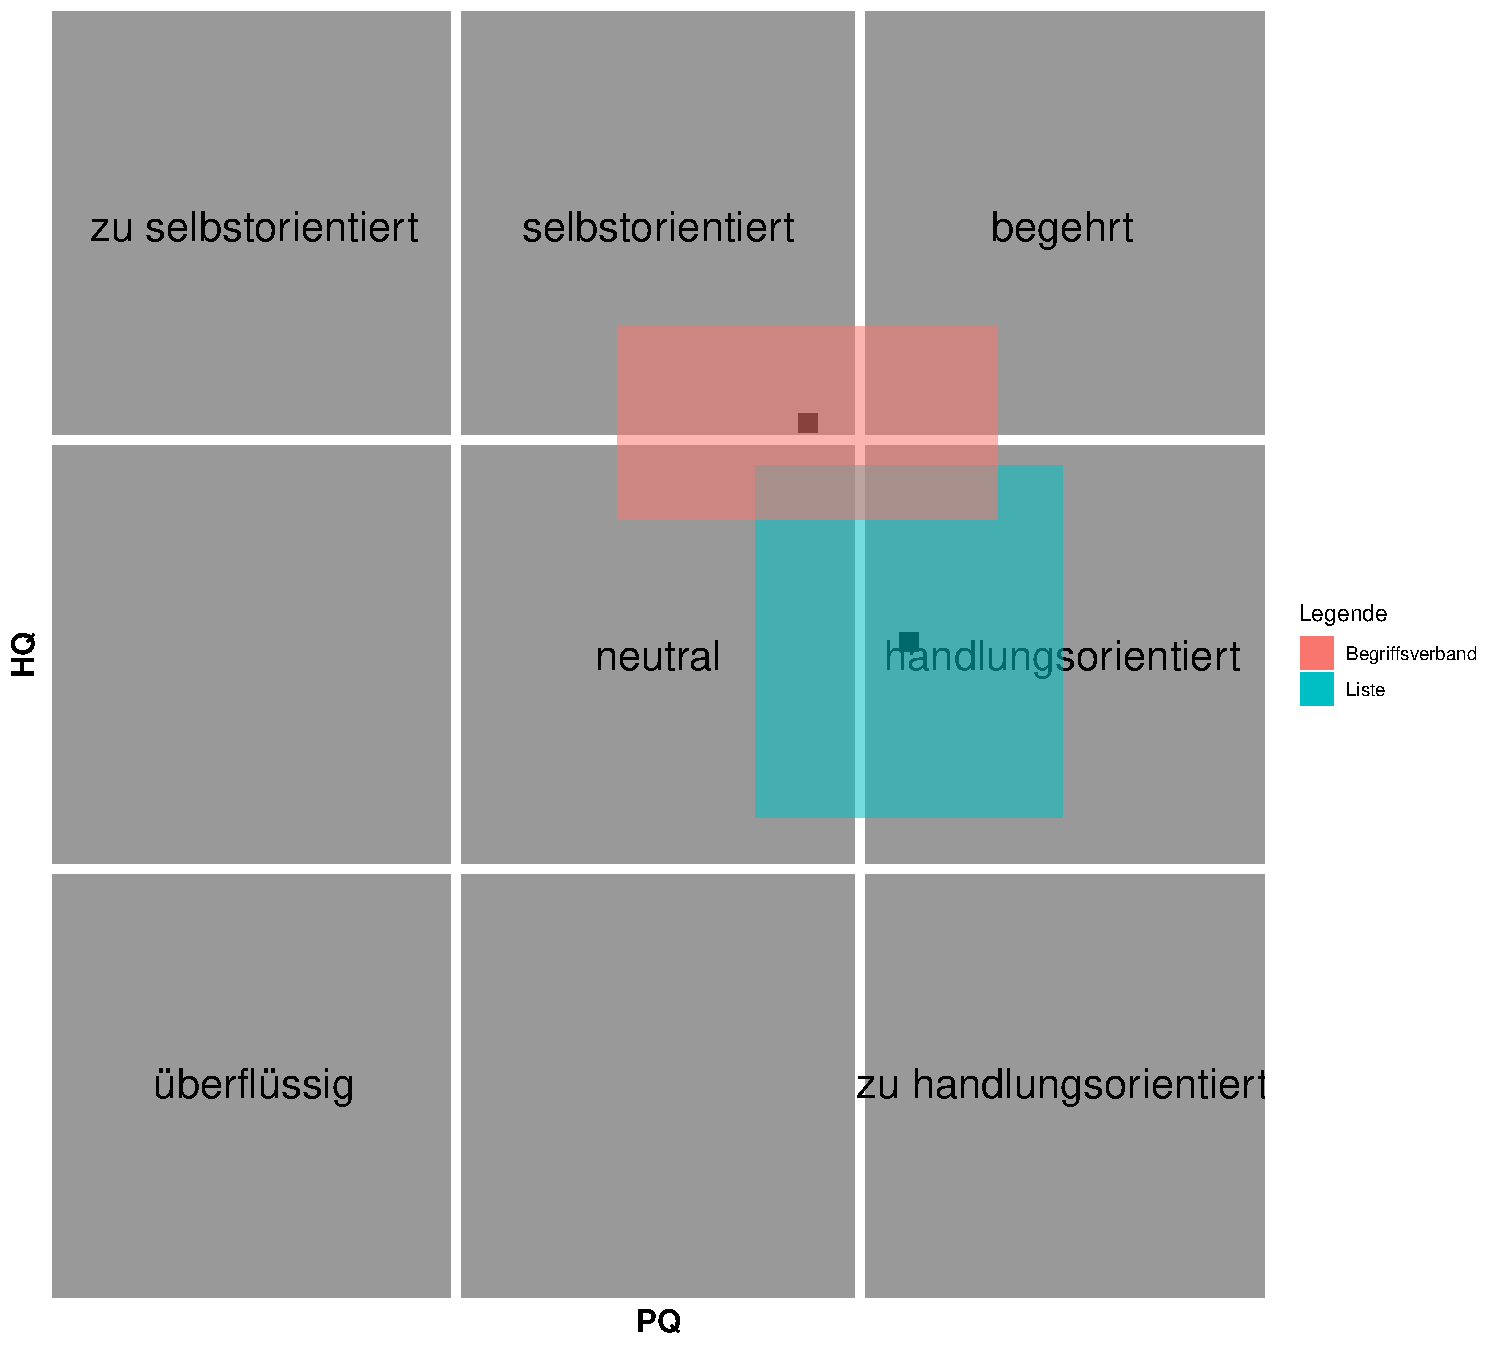
\includegraphics[width=0.7\columnwidth]{figures/attrakdiff-squares.pdf}
    \caption{\label{fig:attrakdiff-squares}AttrakDiff - Portfolio-Darstellung}
\end{figure}

In \autoref{fig:attrakdiff-squares} werden die Ergebnisse des Fragebogens als Portfolio-Darstellung repräsentiert.
Die einzelnen Quadranten stellen dabei die Relation zwischen \ac{PQ} und der \ac{HQ} dar.
Dabei wird ein Produkt als überflüssig bewertet, wenn es eine niedrige \ac{PQ} und eine niedrige \ac{HQ} hat.
Begehrt ist ein Produkt dann, wenn es eine hohe \ac{PQ} und eine hohe \ac{HQ} hat.
Dazwischen existieren weitere Zustände, welche Kompromissformen zwischen beiden Qualitäten darstellen.
Die Spanne für beide Achsen liegt im Intervall von $-3$ bis $3$. \\

Für beide Werte \ac{PQ} und \ac{HQ} sind Konfidenzintervalle als Rechtecke angegeben.
Diese Rechtecke geben mit einer Wahrscheinlichkeit von $95\%$ an, dass in einer weiteren Umfrage die gleiche oder eine ähnliche Bewertung der Produkte erzielt wird.
Die Rechtecke geben zusätzlich an wie unterschiedlich die Testpersonen die Produkte hinsichtlich der \ac{PQ} und der \ac{HQ} bewertet haben.
Der Unterschied zwischen beiden Produkten ist nicht signifikant, da sich die Rechtecke in der horizontalen und vertikalen Achse überlappen.
Ebenfalls können Produkte nicht eindeutig einem Quadranten zugeordnet werden, da die Rechtecke sich nicht vollständig in einem Quadranten befinden.
Dies liegt daran, dass die Testpersonen die Produkte unterschiedlich wahrgenommen und bewertet haben.
Zusätzlich sorgt die geringe Anzahl der Testpersonen für eine geringere Aussagekraft der Ergebnisse.

\begin{figure}[!ht]
    \centering
    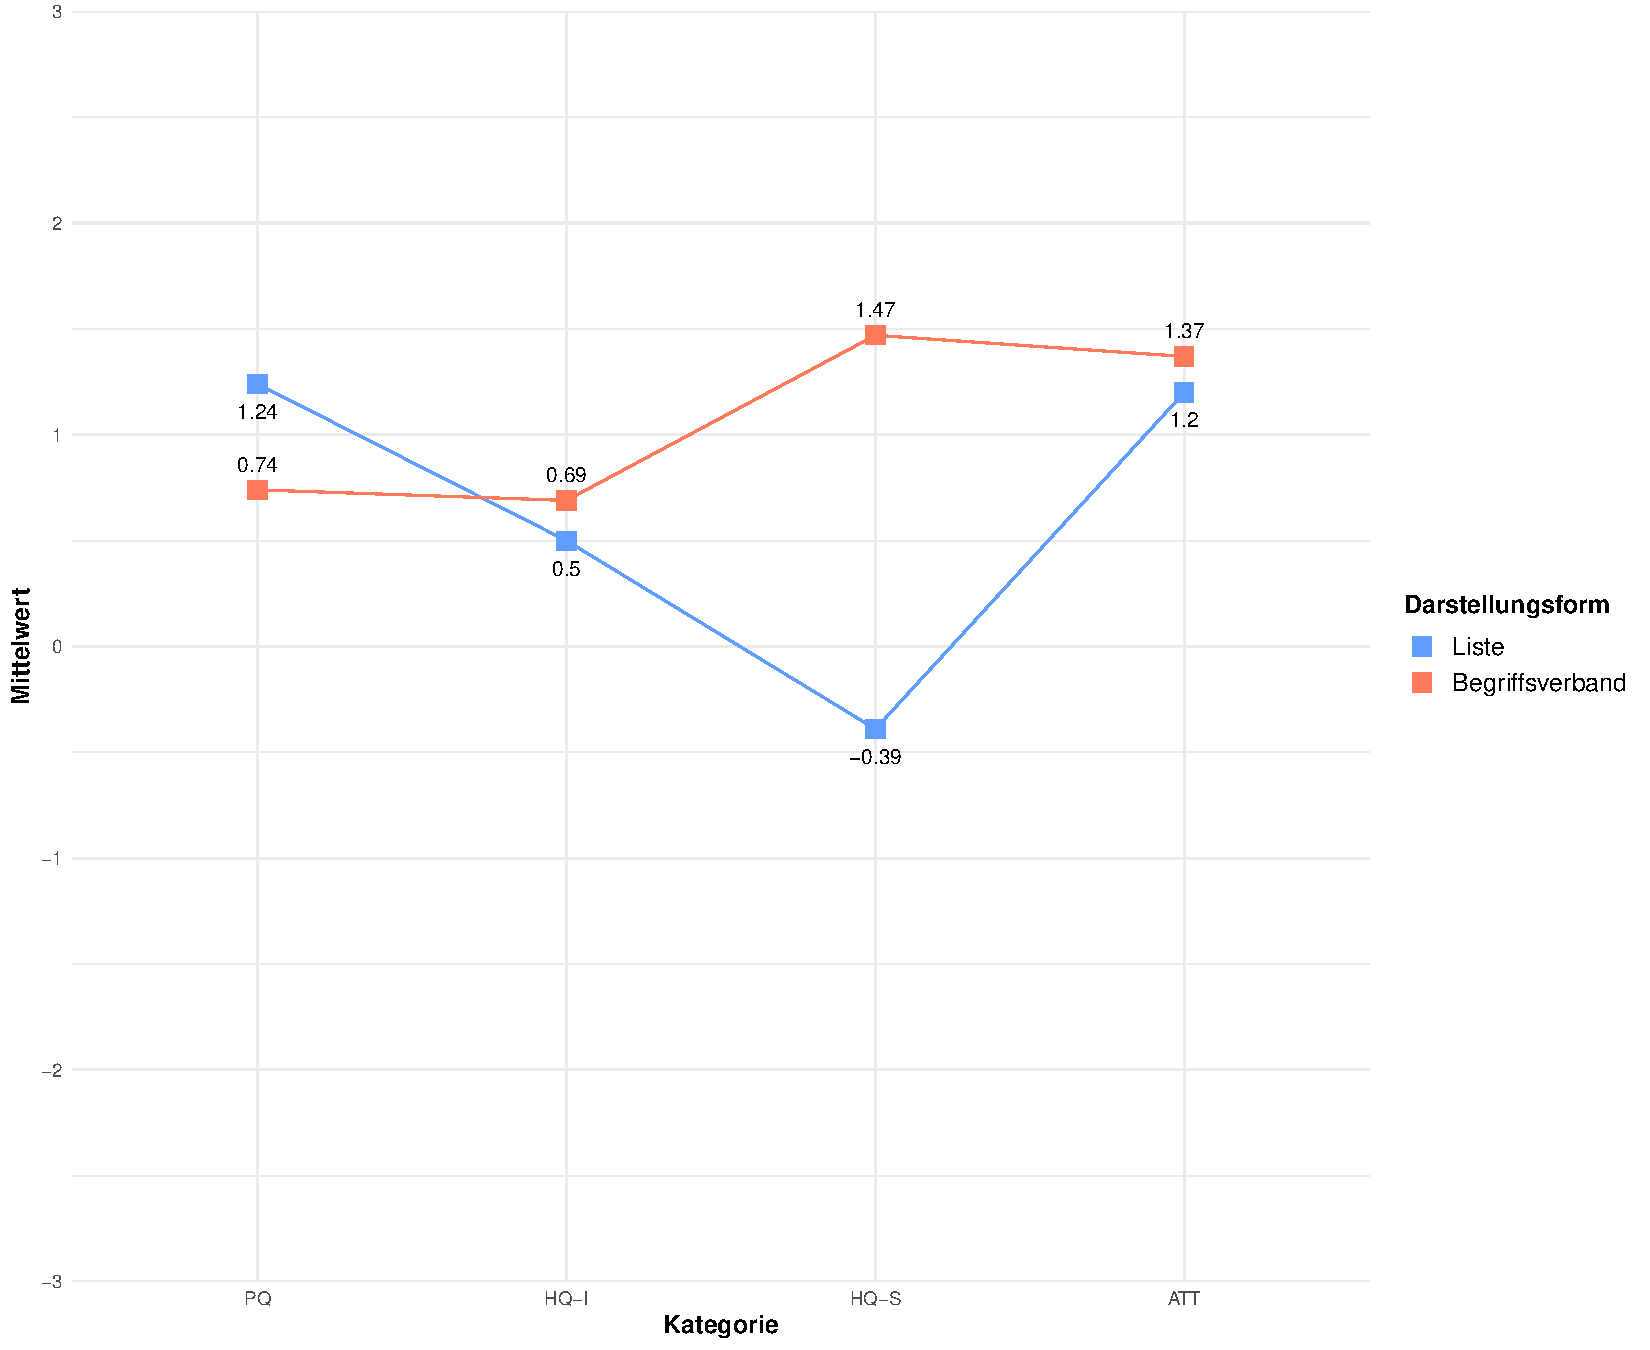
\includegraphics[width=0.7\columnwidth]{figures/attrakdiff-line.pdf}
    \caption{\label{fig:attrakdiff-line}AttrakDiff - Diagramm der Mittelwerte}
\end{figure}

Wenn man die unterschiedlichen Kategorien in \autoref{fig:attrakdiff-line} im direkten Vergleich betrachtet, lässt sich erkennen, dass die Liste nur in der \ac{PQ} im Mittel besser bewertet wurde.
Die \ac{HQ-I}, \ac{HQ-I} und die Attraktivität wurden beim Begriffsverband im Mittel besser bewertet.
Dabei könnte ein Grund für eine bessere \ac{PQ} bei der Listendarstellung sein, dass bereits Vorerfahrungen mit der Handhabung des Produkts bestehen.
Schließlich sind Handlungsziele zu erreichen stark mit dem Vorwissen der Testpersonen verbunden.
Nichtsdestotrotz liegt es ebenfalls nahe, dass die Liste einfacher aufgrund der geringeren Komplexität einfacher zu bedienen ist.\\

Gerade die \ac{HQ-I} und die \ac{HQ-S} sind für die Untersuchung der Masterarbeit von großer Bedeutung.
Schließlich zeigt besonders die \ac{HQ-S}, dass der Begriffsverband das persönliche Wachstum der Testpersonen besser unterstützt als die Listendarstellung.
\textcolor{red}{TODO: Weiter beschreiben}

\subsection{QUESI}
Mithilfe von R wurden die fünf unterschiedlichen Subskalen vom \ac{QUESI}-Fragebogen ausgewertet.
Dafür wurde das arithmetische Mittel $\overline{x}$ und die Standardabweichung SD berechnet.
Da die Antworten auf einer 5-Punkte Likert Skala gegeben wurden, liegt der Mittelwert zwischen $1$ und $5$.
Die daraus resultierenden Werte sind in \autoref{table:quesi-list} und \autoref{table:quesi-fca} dargestellt.
Zusätzlich wurde der \ac{QUESI}-Score über alle Fragen hinweg als Mittelwert berechnet.
Dieser ist ebenfalls in der Tabelle als Score angegeben und dient als Gesamtbewertung der Testpersonen.

\begin{center}
    \begin{table}[!ht]
        \centering
        \begin{tabular}{|l|c|c|c|c|c|c|}
            \hline
                                                 & Arbeitsbelastung & Ziele & Lernen & Vertrautheit & Fehler & Score \\ \hline \hline
            \multicolumn{1}{|c|}{$\overline{x}$} & 4,4              & 4,4   & 4,7    & 4,67         & 5      & 4,61  \\ \hline
            \multicolumn{1}{|c|}{SD}             & 0,93             & 0,81  & 0,79   & 0,66         & 0      & 0,77  \\ \hline
        \end{tabular}
        \caption{QUESI - Liste}
        \label{table:quesi-list}
    \end{table}
\end{center}

Die Mittelwerte für \autoref{table:quesi-list} liegen im Bereich von $4,4$ bis $5$.
Dies deutet darauf hin, dass die Testpersonen die Darstellung als Liste als intuitiv empfunden haben.
Während der Verwendung des Systems gab es keine Probleme mit der Bedienung.
Dies zeigt sich dadurch, dass die Standardabweichung bei der Subskala für Fehler bei $0$ liegt.
Allgemein lässt sich sagen, dass die Antworten der Testpersonen sehr einheitlich waren, da die Standardabweichung bei allen Skalen unter $1$ liegt.

\begin{center}
    \begin{table}[!ht]
        \centering
        \begin{tabular}{|l|c|c|c|c|c|c|}
            \hline
                                                 & Arbeitsbelastung & Ziele & Lernen & Vertrautheit & Fehler & Score \\ \hline \hline
            \multicolumn{1}{|c|}{$\overline{x}$} & 3,23             & 4,37  & 3,27   & 3,83         & 4,25   & 3,76  \\ \hline
            \multicolumn{1}{|c|}{SD}             & 1,41             & 0,76  & 1,39   & 1,29         & 0,85   & 1,27  \\ \hline
        \end{tabular}
        \caption{QUESI - Begriffsverband}
        \label{table:quesi-fca}
    \end{table}
\end{center}

Bei der Auswertung der Antworten bezüglich des Begriffsverbandes lässt sich in \autoref{table:quesi-fca} erkennen, dass die Testpersonen die Darstellung als Begriffsverband als weniger intuitiv empfunden haben.
Ebenfalls waren die Meinungen der Testpersonen unterschiedlicher als bei der Liste.
Dies zeigt sich darin, dass die Standardabweichung bei mehreren Subskalen über $1$ liegt.
Ein Grund hierfür könnte sein, dass die Testpersonen viel unterschiedlichere Erfahrungen mit dem Begriffsverband gemacht haben.
Beweisen lässt sich dies durch die unterschiedlichen Aussagen und Verständnisse zum Begriffsverband in den Interviews.\\

Im direkten Vergleich lässt sich sagen, dass die Ziele mit dem Begriffsverband ähnlich gut erreicht werden können wie mit einer Liste.
Wenn man dies mit der \ac{PQ} aus \autoref{subsec:results-attrakdiff} vergleicht, bestätigen sich die Ergebnisse.
Es wird bei der Listendarstellung zwar eine höhere \ac{PQ} erzielt, jedoch ist diese nicht signifikant.
Ebenfalls bestätigen die Ergebnisse vom \ac{QUESI}-Fragebogen, die Annahme, dass die Vorerfahrung mit einem Produkt die \ac{PQ} beeinflusst.
Gerade die Subskalen für Arbeitsbelastung und Vertrautheit fallen beim Begriffsverband deutlich schlechter aus als bei der Liste.
Dies ist jedoch offensichtlich, wenn die meisten Darstellungsformen im Internet als Liste dargestellt werden.\\

Einige Personen gaben an, dass sie Fehler oder Probleme im Begriffsverband wahrgenommen haben.
Das kann daran liegen, dass die Testpersonen nicht die Möglichkeit hatten, sich ausreichend mit dem Begriffsverband vertraut zu machen.
Aus diesem Grund könnte eine hohe Komplexität und Unverständnis bei der Navigation im Begriffsverband die Ursache für schlechtere Ergebnisse sein.
Dieser Wert lässt sich ebenfalls durch die Interviews und die darin enthaltenen Aussagen bestätigen.
Es wäre jedoch möglich, dass der \ac{QUESI}-Score mit zusätzlichen Erfahrungen und einem verbesserten Tutorial beim Begriffsverband steigen würde.

\subsection{Eigener Fragebogen}
In diesem Abschnitt erfolgt die Auswertung der Ergebnisse des selbst erstellten Fragebogens sowie die Analyse der Aufgaben zur Navigation durch die Prototypen.
Jeder Testperson ist nur die Liste oder eine Variation davon als Darstellungsform für Online-News-Artikel bekannt.
Variationen sind hierbei unendliche Listen oder ein zweidimensionales Kachel-Layout.
Beim zweidimensionalen Kachel-Layout wäre es auch möglich von einem eigenen System zu sprechen, da bei dieser Darstellungsform ebenfalls eine Form der Kategorisierung stattfindet.
Die Kategorisierung erfolgt in diesem Fall jedoch nicht nach den \ac{EC}, sondern nach typischen Rubriken wie Sport oder Wirtschaft.\\

\begin{figure}[!ht]
    \centering
    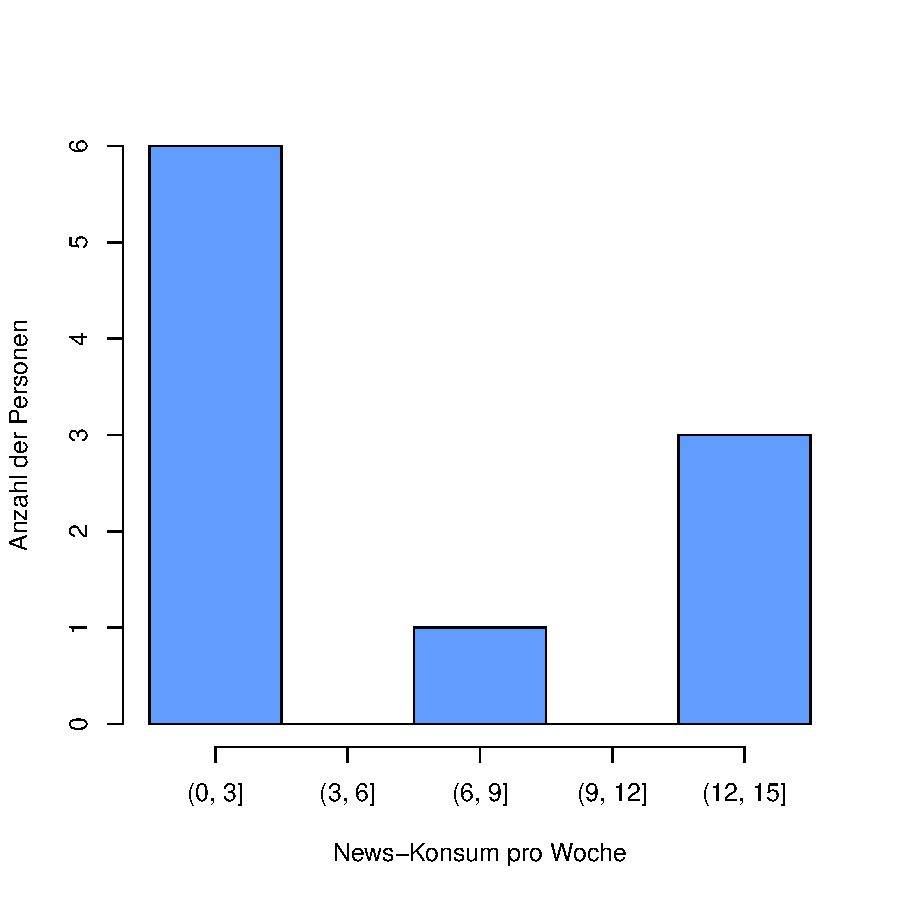
\includegraphics[width=0.6\columnwidth]{figures/news-frequency.pdf}
    \caption{\label{fig:news-consumption}Histogramm - Online-News-Konsum pro Woche}
\end{figure}

\autoref{fig:news-consumption} zeigt die Verteilung der Antworten der Testpersonen bezüglich ihres Online-News-Konsums.
Das Histogramm gibt Aufschluss darüber wie stark das Bedürfnis der Testpersonen nach Online-News ist.
Personen mit einem hohen Konsum können als besonders informiert oder interessiert an Online-News angesehen werden.
Ebenfalls kann diese Zielgruppe als erfahren mit der Nutzung von Online-News betrachtet werden.
Dies fällt besonders auf, wenn man den \ac{QUESI}-Score von Personen mit einem täglichen Konsum mit dem Score von Personen mit geringerem Konsum vergleicht.
Bei der Darstellung als Liste ist der Unterschied zwischen den beiden Gruppen groß genug, um als signifikant angesehen zu werden.
Jedoch ist der Unterschied bei der Darstellung als Begriffsverband deutlich größer.
Die Gruppe mit einem täglichen Konsum weist eine geringere mentale Arbeitsbelastung ($\overline{x} = 3,75$) und eine höhere Vertrautheit ($\overline{x} = 4,17$) auf als die Gruppe mit einem geringeren Konsum ($\overline{x} = 2,89$ und $\overline{x} = 3,61$).
Dadurch ergibt sich für die erste Gruppe auch ein höherer \ac{QUESI}-Score ($\overline{x} = 4,12$, SD=$0,90$) als für die zweite Gruppe ($\overline{x} = 3,51$, SD=$1,42$).


%%% YouTube News 
% P1, 373-375

%%% Kategorisierung wird als gut empfunden, aber Liste bevorzugt
% P1, 390-392
% P5, 227-228 -> Bequemlichkeit

%%% pref. Recommendersystem
% P5, 76-78 -> bewusste Entscheidung für Kategorie
% P5, 85-88 -> Aktive Suche = Google + nicht entscheidungsfreudig

%%% Bei Liste fehlt Zusammenhang 
% P5, 241-244

%%% Filter für Graph
% P6, 147-148

%%% Einarbeitungszeit für Graph
% P7, 127-130

\section{Auswertung}

\section{Ausblick}\label{sec:outlook}
In diesem Abschnitt werden mögliche Erweiterungen für den interaktiven Begriffsverband vorgestellt.
Im Vergleich zum vorherigen \autoref{sec:discussion} werden hier Ansätze vorgestellt, welche bereits zu einem gewissen Teil untersucht wurden.
Alle hier genannten Ansätze sind jedoch nicht umgesetzt oder explizit teil dieser Arbeit.
Stattdessen werden diese Ansätze als mögliche Erweiterungen vorgestellt, welche in zukünftigen Arbeiten oder Iterationen des Prototyps umgesetzt und evaluiert werden können.
Dabei ist zu beachten, dass diese Ansätze nicht vollständig untersucht wurden und daher nur als Ideen zu verstehen sind.
Es gilt diese empirisch zu untersuchen und zu evaluieren, ob diese Ansätze tatsächlich einen Mehrwert für die Nutzenden bieten. \\

\begin{figure}[!ht]
    \centering
    \begin{tikzpicture}
        \definecolor{nodeyellow}{HTML}{FFB50F}
        \definecolor{nodeblue}{HTML}{8EAFF8}

        \draw[line width=1pt] (0,0) arc (180:0:0.25) node[midway,above] {Säugetier};
        \draw[line width=1pt] (0,0) arc (-180:0:0.25) node[midway,below] {Hase};

        \draw[line width=1pt, fill=nodeyellow] (2,0) arc (180:2:0.25) node[midway,above] {Säugetier};
        \draw[line width=1pt, fill=nodeblue] (2,0) arc (-180:2:0.25) node[midway,below] {Hase};
        \draw[line width=1pt] (2,0) -- (2.5,0);

        \draw[fill=nodeyellow] (4,-0.25) rectangle (6,0.25) node[midway] {Säugetier};
        \node at (5,-0.5) {Hase};
    \end{tikzpicture}
    \caption{\label{fig:node-types}Arten der Knotenrepräsentation}
\end{figure}

% Knotentypen
In \autoref{fig:node-types} sind drei verschiedene Möglichkeiten dargestellt Knoten in einem Begriffsverband zu repräsentieren.
Die linke Darstellung repräsentiert einen Knoten, welcher in dieser Form häufig in der Literatur zur \ac{FBA} zu finden ist.
Mittig ist die Darstellung, welche in der Vorstudie und in dieser Arbeit verwendet wurde.
Durch die Verwendung von Farben wird die Zuordnung in Merkmal und Gegenstand visuell unterstützt.
Rechts ist eine weitere Möglichkeit, bei der ein Merkmal in einem Rechteck dargestellt wird und die zugehörigen Gegenstände unterhalb des Rechtecks aufgelistet werden.
In dieser Arbeit wurde zunächst die mittlere Darstellung verwendet, um eine bessere Vergleichbarkeit mit der Vorstudie zu gewährleisten.
Durch das Rechteck hingegen könnte die Zuordnung von Merkmal und Gegenstand deutlicher werden.
In zukünftigen Arbeiten sollte daher untersucht werden, welche Darstellung für die Nutzenden besser geeignet ist.
Eine Interkation, welche zuvor mit dem unteren Halbkreis durchgeführt wurde, würde beim Rechteck entfallen, da das Rechteck keine zwei Interaktionsflächen bietet.
Diese Interaktion ist jedoch nicht zwingend notwendig, da nur die Artikel des angeklickten Knotens angezeigt werden.
Durch die Interaktion mit einem Merkmal wird jedoch der Umfang eines Begriffs aufgeführt, welcher die Artikel des angeklickten Knotens enthält.\\

% Statistik
Durch die Kategorisierung von Artikeln in die \ac{EC} werden neue Möglichkeiten geschaffen, um die Artikel weiter zu analysieren.
Dies schafft zusätzlich weitere Möglichkeiten die Bevölkerung zu informieren.
Es könnten beispielsweise Statistiken erstellt werden, welche Aufschluss über die Anzahl der Artikel geben, welche in die einzelnen Kategorien fallen.
In den Interviews ist aufgefallen, dass die Artikel aus dem Datensatz sich größtenteils positiv bezüglich der Welten der \ac{EC} rechtfertigen.
Wird dies verknüpft mit der Quelle der Artikel, könnte eine Statistik Aufschluss über die Rechtfertigungen eines Mediums geben.
Ebenfalls wäre es möglich, dass die Artikel journalistisch tätiger Personen analysiert werden.
Durch eine sinnvoll gewählte Repräsentation dieser Daten wäre es möglich auf einem Blick zu erkennen, ob eine Redaktion ein breites Spektrum an Welten abdeckt oder sich auf bestimmte Welten und Rechtfertigungen spezialisiert hat.
Für Nutzende könnte dies ein Indikator sein, sich selbst bewusst zu werden, ob das favorisierte Nachrichtenmagazin eine bestimmte Weltsicht vertritt. \\

% Cluster 
Da es journalistischen Standards entspricht, dass Artikel durch ausreichend Quellen belegt werden, entstand die Idee diese Quellen verpflichtend angeben zu lassen.
Dies würde eine weitere Möglichkeit schaffen Nutzende zu informieren und ihnen die Möglichkeit zu geben, sich selbst ein Bild über die Quellen von Artikeln zu machen.
Eine sinnvolle Darstellung dieser Quellen könnte durch die Verwendung von Clustern erreicht werden.
Dabei werden Artikel mit gleichen Quellen in einem Cluster zusammengefasst.
Dieser Ansatz kann verwendet werden, um Zusammenhänge oder Abhängigkeiten zwischen Artikeln zu erkennen.
Nutzende könnten auf diese Weise schnell erkennen, dass mehrere Artikel die gleiche Quelle verwenden.
Durch die Verwendung von Clustern könnten Nutzende erkennen, dass sie sich in einer Filterblase befinden, da sie nur Artikel aus einem Cluster lesen. \\

% Eigene Filterblase
Eine weitere Möglichkeit, um Nutzende zu informieren, wäre die Erstellung einer eigenen Filterblase.
Dabei soll es Nutzenden aber nicht möglich sein, bestimmte Rechtfertigungen auszuschließen.
Stattdessen soll die Filterblase auf Basis der gelesenen Artikel erstellt werden.
Dabei dient diese Filterblase als Möglichkeit, sich selbst bewusst zu werden, welche Inhalte konsumiert wurden.
Durch die Erstellung einer eigenen Filterblase könnte die eigene Weltsicht reflektiert werden.
Für die Erstellung dieser Filterblase ist es notwendig, dass die Artikel, welche gelesen wurden, gespeichert werden.
Dies steht im Konflikt dazu, dass die persönlichen Daten der Nutzenden nicht verarbeitet werden sollen.
Eine Möglichkeit wäre, dass die Artikel lokal im Browser oder auf dem Gerät gespeichert werden.
Auf diese Weise können nur die Nutzenden selbst auf diese Daten zugreifen und ihre eigene Filterblase einsehen.
Dadurch bleibt weiterhin gewährleistet, dass die persönlichen Daten der Nutzenden nicht zum Zweck von Empfehlungen oder anderen Zwecken verarbeitet werden.\\

\section{Fazit}\label{sec:conclusion}
In dieser Arbeit wurde eine Darstellung von News-Artikeln in einem Begriffsverband entwickelt und evaluiert.
Dabei kann die Forschungsfrage, ob die Darstellung von Inhalten in einem Begriffsverband die Auseinandersetzung mit unterschiedlichen Perspektiven fördert, mit Ja beantwortet werden.
Zwar existieren einige Einschränkungen, jedoch konnte an verschiedenen Stellen gezeigt werden, dass das Experiment erfolgreich war.
Durch den Fragebogen AttrakDiff wurde deutlich, dass auch das persönliche Wachstum durch den Begriffsverband gefördert wird.
Aussagen der Testpersonen in den Interviews zufolge konnte zusätzlich gezeigt werden, dass Neugier an anderen Perspektiven geweckt wird.
Dies ist in einer traditionellen Darstellung von Artikeln als Liste nicht möglich, da diese bereits aufgrund des Designs auf wenig Diversität ausgelegt sind.\\

Weiterhin lässt sich festhalten, dass das Tutorial einen positiven Einfluss auf das Verständnis der Darstellung hat.
Zwar weist das Tutorial einige Limitationen auf, jedoch konnte gezeigt werden, dass Testpersonen das Wissen aus dem Tutorial bei der Navigation im Begriffsverband anwenden konnten.
Dies ist ein wichtiger Schritt, um die Darstellung für eine breite Masse zugänglich zu machen.
Schließlich ist es wichtig, dass die Darstellung intuitiv bedienbar ist, damit sie von Nutzenden akzeptiert wird.
Aktuell ist die Darstellung, laut berechneten \ac{QUESI}-Score, noch nicht intuitiv genug, da sie eine zu hohe Arbeitsbelastung für Nutzende darstellt.
Dies ist jedoch nicht verwunderlich, da die Darstellung neuartig ist und sich Nutzende erst an die neue Darstellung gewöhnen müssen.
Trotzdem ist es wichtig, dass die Umgewöhnung möglichst gut unterstützt wird. \\

Dennoch bleibt das Problem der Skalierbarkeit bestehen, was bedeutet, dass weitere Forschung notwendig ist, um die Darstellungsform für eine größere Anzahl an Artikeln zu optimieren.
Ebenfalls ist es notwendig, weitere Experimente durchzuführen, um die Ergebnisse mit einer größeren Stichprobe zu validieren oder neue Darstellungsformen zu erproben.
Insgesamt kann festgehalten werden, dass die Ergebnisse der erprobten Darstellungsform wichtige Erkenntnisse und Einsichten für die Darstellung von News-Artikeln in einem Begriffsverband liefert.
Trotz einiger Einschränkungen konnte gezeigt werden, dass die verwendeten Methoden Potenzial bieten, um die Darstellung hinsichtlich unterschiedlicher Perspektiven zu verbessern.
Durch weitere Forschung und Entwicklung wäre es möglich, dieses Potenzial noch besser auszuschöpfen.


\newpage
\printbibliography

\appendix
\section{Interview Leitfaden}
Dieser Leitfaden dient als Vorlage für das Interview mit den Testpersonen.
Dabei ist die Reihenfolge der Aufgaben abhängig von der Gruppe, in der sich die Testperson befindet.

\subsection{Intro}
Bevor ich das Experiment starte, möchte ich dir kurz den Ablauf und einige wichtige Informationen erklären. 
Zuerst werde ich sicherstellen, dass du über den Datenschutz im Rahmen dieses Experiments informiert bist.
Alle Daten, die ich erfasse, werden anonymisiert und vertraulich behandelt.
Nachdem das Experiment abgeschlossen und die Daten transkribiert wurden, werden diese gelöscht.
Während des Experiments möchte ich dich bitten, deine Gedanken laut auszusprechen.
Das Setting, in dem du dich befindest, lautet wie folgt: \glqq Du interessierst dich für das Thema Elektromobilität und hast dich dazu entschieden, dich darüber zu informieren.\grqq{}

\subsection{Aufgaben - Listenansicht}
Informiere dich zum Thema E-Mobilität.
Navigiere dich wie von anderen News-Websites gewohnt durch die Artikel.
Die hier dargestellte Listenansicht steht stellvertretend für die bereits bekannte Listen im Internet.
\begin{enumerate}
    \item Finde und klicke den Artikel \glqq Strom, Trassen, Verteilernetze\grqq{}.
    \item Finde und klicke den Artikel \glqq Autobauer als Software-Riesen\grqq{}.
    \item Welcher Artikel ist am ähnlichsten zu \glqq Autobauer als Software-Riesen\grqq{}?
    \item Welcher Artikel unterscheidet sich am meisten von \glqq Autobauer als Software-Riesen\grqq{}?
\end{enumerate}

\subsection{Aufgaben - Formale Begriffsanalyse}
Informiere dich zum Thema E-Mobilität.
Verwende dazu das erworbene Wissen aus dem Tutorial, um dich durch die neue Darstellungsform zu navigieren.
\begin{enumerate}
    \item Finde und klicke den Artikel \glqq Harter Schlag für Hersteller Plug-in Prämie fällt weg\grqq{}.
    \item Finde und klicke den Artikel \glqq Deutlich sauberer als gedacht\grqq{}.
    \item Welcher Artikel ist am ähnlichsten zu \glqq Deutlich sauberer als gedacht\grqq{}?
    \item Welcher Artikel unterscheidet sich am meisten von \glqq Deutlich sauberer als gedacht\grqq{}?
\end{enumerate}
\section{Interview Leitfaden \& Fragebogen}
\textcolor{red}{TODO}

\subsection{Intro}
\textcolor{red}{TODO}
\begin{itemize}
    \item Datenschutz
    \item Gedanken laut aussprechen
    \item Setting einleiten
\end{itemize}

\subsection{Setting}
Du interessiert dich für das Thema E-Mobilität und hast dich dazu entschieden, dich darüber zu informieren.

\subsection{Aufgaben - Listenansicht}
Informiere dich zum Thema E-Mobilität.
Navigiere dich wie von anderen News-Websites gewohnt durch die Artikel.
Die hier dargestellte Listenansicht steht stellvertretend für die bereits bekannte Listen im Internet.
\begin{enumerate}
    \item Finde und klicke den Artikel \glqq Strom, Trassen, Verteilernetze\grqq{}.
    \item Finde und klicke den Artikel \glqq Autobauer als Software-Riesen\grqq{}.
    \item Welcher Artikel ist am ähnlichsten zu \glqq Autobauer als Software-Riesen\grqq{}?
    \item Welcher Artikel unterscheidet sich am meisten von \glqq Autobauer als Software-Riesen\grqq{}?
\end{enumerate}

\subsection{Aufgaben - Formale Begriffsanalyse}
Informiere dich zum Thema E-Mobilität.
Verwende dazu das erworbene Wissen aus dem Tutorial, um dich durch die neue Darstellungsform zu navigieren.
\begin{enumerate}
    \item Finde und klicke den Artikel \glqq Harter Schlag für Hersteller Plug-in Prämie fällt weg\grqq{}.
    \item Finde und klicke den Artikel \glqq Deutlich sauberer als gedacht\grqq{}.
    \item Welcher Artikel ist am ähnlichsten zu \glqq Deutlich sauberer als gedacht\grqq{}?
    \item Welcher Artikel unterscheidet sich am meisten von \glqq Deutlich sauberer als gedacht\grqq{}?
\end{enumerate}

\subsection{Fragebogen}
Wir haben uns jetzt mit beiden Darstellungsformen beschäftigt.
Ich habe noch einen weiteren Fragebogen für dich, welchen du mündlich beantworten kannst.
\begin{itemize}
    \item Welche Darstellungsformen für Online-News-Artikel sind dir bekannt?
    \item Wie häufig besuchst du News-Webseiten?
    \item Inwieweit hast du bereits Vorerfahrung zum Thema E-Mobilität?
    \item Könntest du dir vorstellen einer der beiden gezeigten Darstellungsformen persönlich zu nutzen?
    \item Hast du bereits mit Graphen gearbeitet?
    \item Denkst du, dass die dir gezeigte neue Darstellungsform ein diverses Bild der Elektromobilität zeigt?
    \item Wie beeinflusst das Aussehen einer Webseite deine Entscheidung, welche Informationen du liest und wie lange du auf der Seite bleibst?
\end{itemize}

\subsection{Demografische Daten}
Ich habe deine Daten zwar bereits mithilfe vom AttrakDiff-Fragebogen erfasst, aber dieser ist leider etwas ungenau.
Deswegen bitte ich dich, mir noch folgende Daten kurz mitzuteilen.
\begin{itemize}
    \item Alter
    \item Geschlecht
    \item Bildungsstand
    \item Beruf
\end{itemize}

\section{QUESI - Fragebogen}
\textcolor{red}{Inhalt im Hauptteil aufnehmen + cites} \cite{quesi-benchmarks, quesi-short}

\begin{enumerate}
    \item Ich konnte das System, ohne nachzudenken verwenden.
    \item Ich habe erreicht, was ich mit dem System erreichen wollte.
    \item Die Art und Weise, wie das System funktioniert hat, war mir sofort klar.
    \item Ich konnte auf eine mir vertraute Art mit dem System interagieren.
    \item Bei der Verwendung des Systems traten keine Probleme auf.
    \item Das System war nicht kompliziert zu verwenden.
    \item Ich konnte meine Ziele so erreichen, wie ich es mir vorgestellt hatte.
    \item Das System war von Anfang an einfach zu verwenden.
    \item Es war mir immer klar, was ich tun musste, um das System zu verwenden.
    \item Der Prozess des Verwendens des Systems verlief reibungslos.
    \item Ich musste kaum konzentriert auf die Verwendung des Systems achten.
    \item Das System hat mir geholfen meine Ziele vollständig zu erreichen.
    \item Wie das System verwendet wird, war mir sofort klar.
    \item Ich habe automatisch das Richtige getan, um meine Ziele zu erreichen.
\end{enumerate}

\section{STUFF - TODO}\label{sec:stuff}
\textcolor{red}{TODO}

\colorlet{mivertexcolor}{blue}
\colorlet{jivertexcolor}{red}
\colorlet{vertexcolor}{mivertexcolor!50}
\colorlet{bordercolor}{black!80}
\colorlet{linecolor}{gray}
% parameter corresponds to the used valuation function and can be addressed by #1
\tikzset{vertexbase/.style 2 args={semithick, shape=circle, inner sep=2pt, outer sep=0pt, draw=bordercolor},%
    vertex/.style 2 args={vertexbase={#1}{}, fill=vertexcolor!45},%
    mivertex/.style 2 args={vertexbase={#1}{}, fill=mivertexcolor!45},%
    jivertex/.style 2 args={vertexbase={#1}{}, fill=jivertexcolor!45},%
    divertex/.style 2 args={vertexbase={#1}{}, top color=mivertexcolor!45, bottom color=jivertexcolor!45},%
    conn/.style={-, thick, color=linecolor}%
}
\begin{figure}[H]
    \centering
    \begin{adjustbox}{max width=\textwidth}
        \begin{tikzpicture}
            \begin{scope} %for scaling and the like
                \begin{scope} %draw vertices
                    \foreach \nodename/\nodetype/\param/\xpos/\ypos in {%
                            0/vertex//-0.9525641025641018/2.73846153846155,
                            1/jivertex//-0.9102564102564106/6.306410256410267,
                            2/jivertex//-5.155128205128204/7.194871794871805,
                            3/jivertex//3.4333333333333336/7.378205128205138,
                            4/jivertex//-2.6307692307692303/9.352564102564113,
                            5/mivertex//3.546153846153846/11.073076923076933,
                            6/mivertex//-0.7128205128205121/11.143589743589754,
                            7/mivertex//-5.028205128205128/11.214102564102575,
                            8/mivertex//-2.6589743589743584/13.132051282051293,
                            9/vertex//-0.6282051282051277/14.598717948717958
                        } \node[\nodetype={\param}{}] (\nodename) at (\xpos, \ypos) {};
                \end{scope}
                \begin{scope} %draw connections
                    \path (8) edge[conn] (9);
                    \path (3) edge[conn] (5);
                    \path (3) edge[conn] (6);
                    \path (5) edge[conn] (9);
                    \path (0) edge[conn] (3);
                    \path (0) edge[conn] (1);
                    \path (0) edge[conn] (2);
                    \path (1) edge[conn] (5);
                    \path (1) edge[conn] (7);
                    \path (2) edge[conn] (4);
                    \path (2) edge[conn] (7);
                    \path (4) edge[conn] (8);
                    \path (4) edge[conn] (6);
                    \path (7) edge[conn] (8);
                    \path (6) edge[conn] (9);
                \end{scope}
                \begin{scope} %add labels
                    \foreach \nodename/\labelpos/\labelopts/\labelcontent in {%
                    5/above//{Grün},
                    6/above//{Industrie},
                    7/above//{Staat},
                    8/above//{Markt},
                    0/below//{\shortstack{Focus E-Fahrer (E-Auto Förderung 2021) \\ Focus (Neue Elektro-Studie unter der Lupe Jancke/Viehmann) \\ Focus E-Fahrer (Neue E-Auto-Förderung Tesla Tobias Stahl) \\ Focus E-Fahrer (Von wegen nur das Klima retten Tobias Stahl) \\ Focus E-Fahrer (Diesel soll 20 Cent teurer werden Reitberger) \\ Focus E-Fahrer (Rostoffe für E-Auto Akku Reitberger)}},
                    1/below//{Focus (Harter Schlag für Hersteller Plug-in Prämie fällt weg)},
                    2/below//{\shortstack{Focus E-Fahrer (autonom. Fahren Erfolg oder Flop?) \\ Focus E-Fahrer (Auch ohne Berlin-Werk: Schon heute verdient dt. Autoindustrie Kay)}},
                    3/below//{Focus E-Fahrer (Deutlich sauberer als gedacht Tobias Stahl)},
                    4/below//{\shortstack{Focus E-Fahrer (Stromverbrauch: So viel verbraucht ein E-Auto wirklich Siethoff) \\ Focus E-Fahrer (Lohnt sich E-Auto bei den Strompreisen noch?)}},
                    6/below//{Focus E-Fahrer (Revolution oder Wegwerf-Auto? Viehmann)}
                    } \coordinate[label={[\labelopts]\labelpos:{\labelcontent}}](c) at (\nodename);
                \end{scope}
            \end{scope}
        \end{tikzpicture}
    \end{adjustbox}
    \caption{\label{fig:fba-masterthesis}Begriffsverband - Masterarbeit}
\end{figure}

\begin{figure}[H]
    \centering
    \begin{adjustbox}{max width=\textwidth}
        \colorlet{mivertexcolor}{blue}
        \colorlet{jivertexcolor}{red}
        \colorlet{vertexcolor}{mivertexcolor!50}
        \colorlet{bordercolor}{black!80}
        \colorlet{linecolor}{gray}
        % parameter corresponds to the used valuation function and can be addressed by #1
        \tikzset{vertexbase/.style 2 args={semithick, shape=circle, inner sep=2pt, outer sep=0pt, draw=bordercolor},%
            vertex/.style 2 args={vertexbase={#1}{}, fill=vertexcolor!45},%
            mivertex/.style 2 args={vertexbase={#1}{}, fill=mivertexcolor!45},%
            jivertex/.style 2 args={vertexbase={#1}{}, fill=jivertexcolor!45},%
            divertex/.style 2 args={vertexbase={#1}{}, top color=mivertexcolor!45, bottom color=jivertexcolor!45},%
            conn/.style={-, thick, color=linecolor}%
        }
        \begin{tikzpicture}
            \begin{scope} %for scaling and the like
                \begin{scope} %draw vertices
                    \foreach \nodename/\nodetype/\param/\xpos/\ypos in {%
                            0/vertex//0.061685823754787705/1.3448275862068968,
                            1/divertex//-1.0/3.0,
                            2/divertex//1.4103448275862052/3.9747126436781617,
                            3/divertex//-1.0/5.0,
                            4/vertex//-0.0057471264367841/6.4107279693486605
                        } \node[\nodetype={\param}{}] (\nodename) at (\xpos, \ypos) {};
                \end{scope}
                \begin{scope} %draw connections
                    \path (1) edge[conn] (3);
                    \path (3) edge[conn] (4);
                    \path (2) edge[conn] (4);
                    \path (0) edge[conn] (1);
                    \path (0) edge[conn] (2);
                \end{scope}
                \begin{scope} %add labels
                    \foreach \nodename/\labelpos/\labelopts/\labelcontent in {%
                    1/above//{Staat},
                    2/above//{Grün},
                    3/above//{Markt},
                    4/above//{Industrie},
                    0/below//{\shortstack{Focus E-Fahrer (E-Auto Förderung 2021) \\ Focus E-Fahrer (Neue E-Auto-Förderung Tesla Tobias Stahl) \\ Focus E-Fahrer (Von wegen nur das Klima retten Tobias Stahl) \\ Focus E-Fahrer (Rohstoffe für E-Auto Akku Reitberger) \\ Focus E-Fahrer (Diesel soll 20 Cent teurer werden Reitberger)}},
                    1/below//{\shortstack{Focus E-Fahrer (autonom. Fahren Erfolg oder Flop?) \\ Focus E-Fahrer (Auch ohne Berlin-Werk: Schon heute verdient dt. Autoindustrie Kay)}},
                    2/below//{Focus E-Fahrer (Deutlich sauberer als gedacht Tobias Stahl)},
                    3/below//{\shortstack{Focus E-Fahrer (Stromverbrauch: So viel verbraucht ein E-Auto wirklich Siethoff) \\ Focus E-Fahrer (Lohnt sich E-Auto bei den Strompreisen noch?)}},
                    4/below//{\shortstack{Focus E-Fahrer (Revolution oder Wegwerf-Auto? Viehmann) \\ Focus E-Fahrer (Auto-Bloggerin nimmt Tesla Modell auseinander Albrecht)}}
                    } \coordinate[label={[\labelopts]\labelpos:{\labelcontent}}](c) at (\nodename);
                \end{scope}
            \end{scope}
        \end{tikzpicture}
    \end{adjustbox}
    \caption{\label{fig:fba-smaller}Reduzierter Begriffsverband - Vorstudie}
\end{figure}

\end{document}
